% Options for packages loaded elsewhere
\PassOptionsToPackage{unicode}{hyperref}
\PassOptionsToPackage{hyphens}{url}
\PassOptionsToPackage{dvipsnames,svgnames*,x11names*}{xcolor}
%
\documentclass[
  english]{revcoles}
\usepackage{lmodern}
\usepackage{amssymb,amsmath}
\usepackage{ifxetex,ifluatex}
\ifnum 0\ifxetex 1\fi\ifluatex 1\fi=0 % if pdftex
  \usepackage[T1]{fontenc}
  \usepackage[utf8]{inputenc}
  \usepackage{textcomp} % provide euro and other symbols
\else % if luatex or xetex
  \usepackage{unicode-math}
  \defaultfontfeatures{Scale=MatchLowercase}
  \defaultfontfeatures[\rmfamily]{Ligatures=TeX,Scale=1}
\fi
% Use upquote if available, for straight quotes in verbatim environments
\IfFileExists{upquote.sty}{\usepackage{upquote}}{}
\IfFileExists{microtype.sty}{% use microtype if available
  \usepackage[]{microtype}
  \UseMicrotypeSet[protrusion]{basicmath} % disable protrusion for tt fonts
}{}
\makeatletter
\@ifundefined{KOMAClassName}{% if non-KOMA class
  \IfFileExists{parskip.sty}{%
    \usepackage{parskip}
  }{% else
    \setlength{\parindent}{0pt}
    \setlength{\parskip}{6pt plus 2pt minus 1pt}}
}{% if KOMA class
  \KOMAoptions{parskip=half}}
\makeatother
\usepackage{xcolor}
\IfFileExists{xurl.sty}{\usepackage{xurl}}{} % add URL line breaks if available
\IfFileExists{bookmark.sty}{\usepackage{bookmark}}{\usepackage{hyperref}}
\hypersetup{
  colorlinks=true,
  linkcolor=blue,
  filecolor=Maroon,
  citecolor=Blue,
  urlcolor=blue,
  pdfcreator={LaTeX via pandoc}}
\urlstyle{same} % disable monospaced font for URLs
\usepackage{graphicx}
\makeatletter
\def\maxwidth{\ifdim\Gin@nat@width>\linewidth\linewidth\else\Gin@nat@width\fi}
\def\maxheight{\ifdim\Gin@nat@height>\textheight\textheight\else\Gin@nat@height\fi}
\makeatother
% Scale images if necessary, so that they will not overflow the page
% margins by default, and it is still possible to overwrite the defaults
% using explicit options in \includegraphics[width, height, ...]{}
\setkeys{Gin}{width=\maxwidth,height=\maxheight,keepaspectratio}
% Set default figure placement to htbp
\makeatletter
\def\fps@figure{htbp}
\makeatother
\setlength{\emergencystretch}{3em} % prevent overfull lines
\providecommand{\tightlist}{%
  \setlength{\itemsep}{0pt}\setlength{\parskip}{0pt}}
\setcounter{secnumdepth}{-\maxdimen} % remove section numbering

\setcounter{tocdepth}{5}
\setcounter{secnumdepth}{5}
 %Esto quita el punto final en la numeracion de cada seccion
\usepackage{tocloft}

\usepackage{titlesec}

\titleformat{\subsection}
{\large\bfseries}{\thesubsection}{0.5em}{}
\titleformat{\subsubsection}
{\normalsize\bfseries}{\thesubsubsection}{0.5em}{}
\titleformat{\paragraph}
{\normalsize\bfseries}{\theparagraph}{0.5em}{}
\renewcommand\cftsecaftersnum{}
\renewcommand\thesection{\arabic{section}}
\renewcommand\thesubsection{\thesection.\arabic{subsection}}

\usepackage{scalerel}
\usepackage{tikz}
\usetikzlibrary{svg.path}

\definecolor{orcidlogocol}{HTML}{A6CE39}
\tikzset{
  orcidlogo/.pic={
    \fill[orcidlogocol] svg{M256,128c0,70.7-57.3,128-128,128C57.3,256,0,198.7,0,128C0,57.3,57.3,0,128,0C198.7,0,256,57.3,256,128z};
    \fill[white] svg{M86.3,186.2H70.9V79.1h15.4v48.4V186.2z}
                 svg{M108.9,79.1h41.6c39.6,0,57,28.3,57,53.6c0,27.5-21.5,53.6-56.8,53.6h-41.8V79.1z M124.3,172.4h24.5c34.9,0,42.9-26.5,42.9-39.7c0-21.5-13.7-39.7-43.7-39.7h-23.7V172.4z}
                 svg{M88.7,56.8c0,5.5-4.5,10.1-10.1,10.1c-5.6,0-10.1-4.6-10.1-10.1c0-5.6,4.5-10.1,10.1-10.1C84.2,46.7,88.7,51.3,88.7,56.8z};
  }
}

\newcommand\orcidicon[1]{\href{https://orcid.org/#1}{\mbox{\scalerel*{

\begin{tikzpicture}[yscale=-1,transform shape]
\pic{orcidlogo};
\end{tikzpicture}
}{|}}}}

\usepackage{hyperref}

%Paquetes adicionales para ecuaciones, símbolos y figuras
\usepackage{amssymb}
\usetikzlibrary{babel,positioning,shapes.multipart,calc,arrows.meta}
\usepackage{booktabs}
\usepackage{longtable}
\usepackage{array}
\usepackage{multirow}
\usepackage{wrapfig}
\usepackage{float}
\usepackage{colortbl}
\usepackage{pdflscape}
\usepackage{tabu}
\usepackage{threeparttable}
\usepackage{threeparttablex}
\usepackage[normalem]{ulem}
\usepackage{makecell}
\usepackage{xcolor}
\newlength{\cslhangindent}
\setlength{\cslhangindent}{1.5em}
\newenvironment{cslreferences}%
  {\setlength{\parindent}{0pt}%
  \everypar{\setlength{\hangindent}{\cslhangindent}}\ignorespaces}%
  {\par}

\author{}
\date{\vspace{-2.5em}}

\begin{document}

\begin{title}
\title[maintitle = Kurtosis effects on Estimating Structural Equation Models Over Different Sample Sizes,
       secondtitle = Efectos de la Kurtosis en la estimación de Modelos de Ecuaciones Estructurales bajo distintos tamaños de muestra,
       shorttitle = Short title in English
]
\end{title}

\begin{authors}
\author[firstname = César,
        surname = Gamboa-Sanabria,
        numberinstitution = 1,
        affiliation = {School of Statistics, University of Costa Rica}, 
        email = info@cesargamboasanabria.com] \orcidicon{0000-0001-6733-4759}\,
\author[firstname = Andrés,
        surname = Arguedas-Leiva,
        numberinstitution = 1,
        affiliation = {School of Statistics, University of Costa Rica}, 
        email = andres.arguedasleiva@ucr.ac.cr] \orcidicon{0000-0001-6299-052X}
\end{authors}

\begin{institutions}
     \institute[subdivision = {School of Statistics},
                division = Faculty of Economical Sciences,
                institution = University of Costa Rica,
                city = San José,
                country = Costa Rica]
\end{institutions}

\begin{mainabstract}
 Insert your abstract here.
\keywords{SEM, simulation, kurtosis, lavaan}
\end{mainabstract}

\begin{secondaryabstract}
Inserte su resumen aquí.
\keywords{SEM, simulación, kurtosis, lavaan}
\end{secondaryabstract}

\section{Introduction}

\subsection{Antecedentes}

Los Modelos de Ecuaciones Estructurales (en adelante SEM, por sus siglas
en inglés) representan un compendio de métodos estadísticos que buscan
estimar y examinar las relaciones causales existentes entre varias
mediciones fácilmente observables con conceptos más abstractos,
denominados constructos, que no pueden ser medidos ni analizados de
manera directa. Los SEM trabajan de una manera similar a los modelos de
regresión más clásicos, pero representan una mejora pues analizan las
relaciones causales lineales entre las variables involucradas al mismo
tiempo que los errores de medición (Beran \& Violato,
\protect\hyperlink{ref-Beran2010}{2010}). Para medir estas relaciones
causales, los SEM cuentan con dos grandes componentes: 1) el modelo
estructural, cuya función es cuantificar las relaciones causales
presentes entre cada uno de los constructos planteados desde la teoría;
y 2) un modelo de medición, cuyo objetivo último es brindar una
descripción acerca de cuáles son los indicadores que sirven para medir
los constructos en cuestión (Kaplan,
\protect\hyperlink{ref-Kaplan2012}{2012}).

Los SEM están presentes en multitud de campos de investigación como la
psicología, la sociología, las políticas públicas y ciencias
relacionadas a la familia (Tarka,
\protect\hyperlink{ref-Tarka2018}{2018}), además, trabajos como el de
Golob (\protect\hyperlink{ref-Golob2003}{2003}) muestran la aplicación
de los SEM en fenómenos económicos, o bien en investigación de mercados
como sugieren los trabajos de Bagozzi
(\protect\hyperlink{ref-Bagozzi1980}{1980}) y Chin, Peterson, \& Brown
(\protect\hyperlink{ref-Chin2008}{2008}). Según Beran \& Violato
(\protect\hyperlink{ref-Beran2010}{2010}), la cantidad de referencias a
SEM en 1994 fueron de 164, aumentaron a 343 en el 2000 y llegaron a 742
en el 2009, lo cual es una señal de que muchos investigadores alrededor
del mundo están mostrando cada vez más interés en este tipo de estudios,
pues representan una potente herramienta para la investigación partiendo
de la teoría sustantiva que poseen los diversos estudios.

Uno de los principales campos de aplicación de los SEM son las ciencias
sociales, pues se busca explicar y/o predecir con un grado de validez el
comportamiento específico de una o varias personas en grupo. Teniendo
siempre en consideración (aunque de forma limitada) las condiciones que
afectan a cada individuo involucrado en el estudio, así como las
características propias de su entorno, los grupos de investigación
pueden definir factores, además de las relaciones latentes y de
causalidad entre ellos que se encuentran implícitas en el comportamiento
humano. Este tipo de investigaciones permite entender los fenómenos no
solo de forma descriptiva, sino que es posible también determinar
relaciones de causalidad (Tarka,
\protect\hyperlink{ref-Tarka2018}{2018}).

Las variables indicadoras, las cuales se utilizan para construir los
llamados constructos, pueden llegar a comportarse de manera muy diversa.
Las ciencias sociales, al trabajar con seres humanos, es común trabajar
con variables cuyo comportamiento es particularmente irregular,
presentando valores muy distintos entre los sujetos de estudio,
generando de esta manera que los indicadores de manera multivariada no
sigan una distribución normal, lo cual representa un supuesto
fundamental al trabajar con SEM (Sura-Fonseca,
\protect\hyperlink{ref-SuraFonseca2020}{2020}), esta condición puede
afectar negativamente la estimación del modelo y sus estadísticos de
bondad de ajuste, llevando a pérdidas en la potencia (Foss, Jreskog, \&
Olsson, \protect\hyperlink{ref-Foss2011}{2011}) o al caso de descartar
modelos que podrían ser adecuados solo por presentar un mal ajuste
(Andreassen, Lorentzen, \& Olsson,
\protect\hyperlink{ref-Andreassen2006}{2006}). El no cumplimiento de
este supuesto puede deberse, entre otras cosas, a medidas
particularmente altas o bajas de una medida estadística en específico:
la kurtosis.

\subsection{El problema}

Si al trabajar con un SEM no se cumple el supuesto de normalidad
multivariada y además el modelo se estima vía máxima verosimilitud, que
al día de hoy se mantiene como el método de estimación más extendido y
popular, podría cometerse el error de sobreestimar el estadístico
chi-cuadrado, el cual sirve de referencia para conocer la magnitud de la
diferencia entre la matriz de covariancias estimadas por el modelo con
la obtenida en la muestra. Lo anterior suele llevar a rechazar modelos
que en realidad resumen bien la realidad para dar una mejor explicación
del por qué sucede un fenómeno, y además a la subestimación de los
errores asociados a los parámetros, lo cual genera interpretaciones
inadecuadas en lo referente a la significancia estadística de las
relaciones planteadas por el modelo teórico.

Por otro lado, es posible toparse con conjuntos de datos que, en su
conjunto, no presenten una distribución normal multivariada debido a la
muy alta o muy baja concentración de datos alrededor de la zona central
de su distribución. Este comportamiento se mide mediante un estadístico
llamado kurtosis, que describe qué tan aplanada o empinada es la
distribución, dependiendo de este estadístico, es posible saber si los
datos atentan contra la presencia de una distribución normal. Trabajos
como el de Sura-Fonseca (\protect\hyperlink{ref-SuraFonseca2020}{2020})
o el de Andreassen et~al. (\protect\hyperlink{ref-Andreassen2006}{2006})
han abierto espacios de investigación para esta temática

Considerar distintos niveles de kurtosis permite conocer el impacto que
esta medida tiene sobre las estimaciones de un SEM dependiendo del
tamaño de muestra utilizado (Muthen \& Kaplan,
\protect\hyperlink{ref-Muthen1992}{1992}).

\subsection{Objetivos del estudio}

La presente investigación busca estudiar el efecto que tienen distintos
niveles de kurtosis en varios tamaños de muestra sobre las estimaciones
de un SEM. Para ello, se ha tomado tomado como base un estudio de la
Universidad de California (Gao, Mokhtarian, \& Johnston,
\protect\hyperlink{ref-Gao2008}{2008}), por ser uno de los trabajos más
recientes en cuanto a planteamiento de tamaños de muestra y kurtosis
para la simulación de datos multivariados. Se plantean los siguientes
objetivos:

\subsubsection{Objetivo general}

Comparar mediante un estudio de simulación los efectos en las
estimaciones de cargas factoriales y medidas de ajuste de modelos de
ecuaciones estructurales estimados mediante máxima verosimilitud en
presencia de variables observadas con niveles de kurtosis de 0, 0.62,
6.65, 21.41 y 13.92 en tamaños de muestra de 50, 100, 120, 200 y 300.

\subsubsection{Objetivos específicos}

\textbf{1)} Definir como modelo poblacional el obtenido por Sura-Fonseca
(\protect\hyperlink{ref-SuraFonseca2020}{2020}) con dos variables
exógenas y una endógena con tres variables indicadoras cada uno como
modelo de referencia teórico cuyas cargas factoriales se utilizarán para
la generación de los datos simulados.

\textbf{2)} Medir el posible sesgo causado en la estimación de los
modelos mediante el estadístico chi-cuadrado del modelo y la raíz del
cuadrado medio de error de aproximación (RMSEA), la raíz de residuos de
cuadrado medio estandarizado (SRMR) y el índice de bondad de ajuste
(GFI).

\textbf{3)} Comparar los valores poblacionales de las cargas factoriales
con los obtenidos en las simulaciones.

\textbf{4)} Publicar en una revista científica con revisión por pares el
manuscrito final, en forma de un artículo científico.

\subsection{Metodología de la investigación}

De esta manera, el presente estudio consiste en en simular datos no
normales multivariados con diferentes tamaños de muestra y kurtosis para
la estimación de SEM tomando como punto modelo de referencia el obtenido
por Sura-Fonseca (\protect\hyperlink{ref-SuraFonseca2020}{2020}) para
las habilidades cuantitativas, el cual consiste en dos variables
exógenas y una endógena. Se realizaron 2000 conjuntos de datos para cada
escenario de simulación y se comparan las estimaciones de tanto de las
cargas factoriales como de varios estadísticos de bondad de ajuste que
serán descritos más adelante.

\section{Methodology}

\subsection{Generación de datos con kurtosis}

Los datos fueron simulados mediante la función \texttt{simulateData()}
del paquete \texttt{lavaan} (Rosseel,
\protect\hyperlink{ref-lavaan}{2012}), el cual utiliza el método
propuesto por Vale \& Maurelli (\protect\hyperlink{ref-Vale1983}{1983})
para la simulación de datos no normales multivariados. Este método,
comúnmente conocido como VM, se basa en el método propuesto por
Fleishman (\protect\hyperlink{ref-Fleishman1978}{1978}), el cual, con
base en una variable aleatoria distribuida como una normal estándar,
permite simular una variable con un promedio, variancia, asimetría y
kurtosis dada. El método VM permite especificar, adicionalmente,
correlaciones entre las variables a estimar. Para utilizar el método de
Fleishman, para generar una cierta variable aleatoria \(Y\), se utiliza
la siguiente ecuación:

\begin{equation} \label{eq:defY}
  Y = a + bX + cX^2 + d X^3
\end{equation}

donde \(X \sim \mathcal{N} (0,1)\). Es decir, se puede generar una
variable no normal \(Y\), con sus primeros cuatro momentos iguales a
valores especificados, con base en los valores \(a\), \(b\), \(c\) y
\(d\) de la ecuación \ref{eq:defY}, con base en una variable normal
estándar \(X\) hasta su tercer potencia. Luego, para poder obtener los
valores de \(a\), \(b\), \(c\) y \(d\), se necesitan resolver las
siguientes ecuaciones de forma simultánea:

\begin{align*}
  b^2 + 6bd + 2c^2 + 15d^2 -1 & = 0 \\
  2c (b^2 + 24bd + 105d^2 + 2) - \gamma_1 & = 0 \\
  24 \left(bd + c^2 (1 + b^2 + 28bd) + d^2 (12 + 48bd + 141c^2 + 225d^2) \right) - \gamma_2 & = 0
\end{align*}

donde \(\gamma_1\) es la asimetría deseada y \(\gamma_2\) es la kurtosis
deseada, además se define \(a = -c\). Con base en las constantes
calculadas \(a\), \(b\), \(c\) y \(d\), además de una variable normal
estándar, se puede simular variables no normales. Para poder generalizar
el método de Fleishman a variables aleatorias multivariantes, Vale y
Maurelli proponen una generalización. Esta se basa, para el caso
bivariado, en la generación de dos variables aleatorias independientes,
\(X_1, X_2 \sim \mathcal{N} (0,1)\), para la cuales se obtienen las
constantes \(a\), \(b\), \(c\) y \(d\), para cada una de dichas
variables, como se describe en el método de Fleishman, obteniendo así el
vector \(w^\prime_1 = (a_1, b_1, c_1, d_1)\), para el caso de \(X_1\), y
el vector \(w^\prime_2 = (a_2, b_2, c_2, d_2)\), para el caso de
\(X_2\). Además, se definen los vectores
\(x_1^\prime = (1, X_1, X_1^2, X_1^3)\) y
\(x_2^\prime = (1, X_2, X_2^2, X_2^3)\). Por lo tanto, se pueden crear
variables no normales, \(Y_1\) y \(Y_2\), como:

\begin{align*}
  Y_1 & = w_1^\prime x_1 \\
  Y_2 & = w_2^\prime x_2
\end{align*}

donde se puede verificar que:

\begin{align*}
  r_{Y_1, Y_2} = & \rho_{X_1, X_2} (b_1 b_2 + 3b_1 d_2 + 3d_1 b_2 + 9 d_1 d_2) \\
  & + \rho_{X_1, X_2}^2 (2 c_1 c_2) + \rho_{X_1, X_2}^3 (6 d_1 d_2)
\end{align*}

Y resolviendo esta ecuación en términos de \(\rho_{X_1, X_2}\) se puede
obtener una matriz de correlaciones para generar datos normales
multivariados, que pueden ser transformados en variables no normales
mediante el método de Fleishman.

\subsection{Modelo a estimar}

El modelo teórico utilizada para realizar las simulaciones es el
presentado por Sura-Fonseca
(\protect\hyperlink{ref-SuraFonseca2020}{2020}), basado en datos de 155
estudiantes de la Universidad de Costa Rica, obtenidos de la Prueba de
Habilidades Cuantitativas (PHC) del Instituto de Investigaciones
Psicológicos (IIP) de dicha universidad y de un cuestionario
autoadministrado aplicado a estos estudiantes. El modelo estimado está
compuesto por dos variables exógenas (capital y habilidades
cuantitativas) y una variable endógena (habilidades visoespaciales). Con
respecto a estas variables: el capital se refiere al acceso y tenencia
de ciertos bienes en los hogares de los estudiantes; las habilidades
cuantitativas se refieren a la puntuación de los estudiantes en la
prueba mencionada anteriormente; y las habilidades visoespaciales se
refieren a la capacidad de los estudiantes para poder trabajar con
objetos tridimensionales abstractos y poder manipularlos en la
imaginación. Para cada una de estas variables latentes, se utilizó el
método de parcelas para obtener tres variables indicadoras para cada uno
de los constructos. Los resultados de la estimación de dicho modelo,
presentados por Sura-Fonseca
(\protect\hyperlink{ref-SuraFonseca2020}{2020}), se presentan en la
Figura \ref{fig:mod_teorico}.

\begin{figure}[!h]
\centering
\caption{Modelo estimado sobre las habilidades cuantitativas}
\label{fig:mod_teorico}
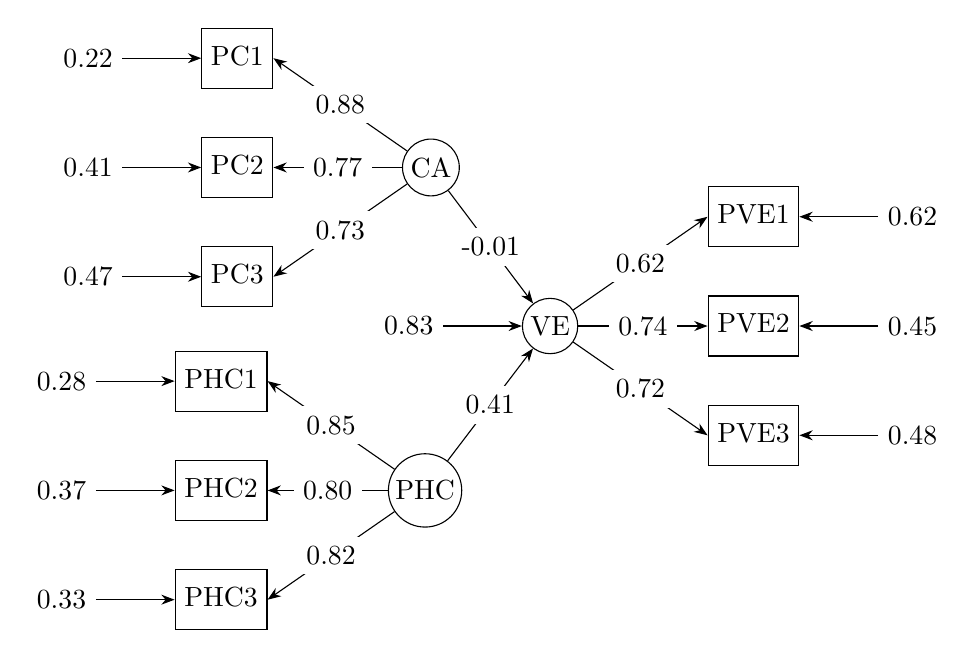
\begin{tikzpicture}
        [
    basic/.style={draw, text centered},
    circ/.style={basic, circle, minimum size=2em, inner sep=1.5pt},
    rect/.style={basic, text height=1em, text depth=.5em, minimum width=1.5em},
    >={Stealth[]}
    ]

    % Variables latentes
    \node [circ] (ve) {VE};
    \node [circ, above left=1.5cm and 1cm of ve] (ca) {CA};
    \node [circ, below left=1.5cm and 1cm of ve] (phc) {PHC};
    \draw [->] (ca) -- node[fill=white] {-0.01} (ve);
    \draw [->] (phc) -- node[fill=white] {0.41} (ve);
    % Variancia de VE
    \node [left=of ve] (delta) {0.83};
    \draw [->] (delta) -- (ve);
    % Variables indicadoras de VE
    \node [rect, above right=1cm and 2cm of ve.center] (pve1) {PVE1};
    \node [rect, right=2cm of ve.center] (pve2) {PVE2};
    \node [rect, below right=1cm and 2cm of ve.center] (pve3) {PVE3};
    \draw [->] (ve) -- node[fill=white] {0.62} (pve1.west);
    \draw [->] (ve) -- node[fill=white] {0.74} (pve2.west);
    \draw [->] (ve) -- node[fill=white] {0.72} (pve3.west);
    % Variancia de variables indicadoras de VE
    \node [right=of pve1] (epve1) {0.62};
    \node [right=of pve2] (epve2) {0.45};
    \node [right=of pve3] (epve3) {0.48};
    \draw [->] (epve1) -- (pve1);
    \draw [->] (epve2) -- (pve2);
    \draw [->] (epve3) -- (pve3);
    % Variables indicadoras de CA
    \node [rect, above left=1cm and 2cm of ca.center] (pc1) {PC1};
    \node [rect, left=2cm of ca.center] (pc2) {PC2};
    \node [rect, below left=1cm and 2cm of ca.center] (pc3) {PC3};
    \draw [->] (ca) -- node[fill=white] {0.88} (pc1.east);
    \draw [->] (ca) -- node[fill=white] {0.77} (pc2.east);
    \draw [->] (ca) -- node[fill=white] {0.73} (pc3.east);
    % Variancia de variables indicadoras de CA
    \node [left=of pc1] (epc1) {0.22};
    \node [left=of pc2] (epc2) {0.41};
    \node [left=of pc3] (epc3) {0.47};
    \draw [->] (epc1) -- (pc1);
    \draw [->] (epc2) -- (pc2);
    \draw [->] (epc3) -- (pc3);
    % Variables indicadoras de PHC
    \node [rect, above left=1cm and 2cm of phc.center] (phc1) {PHC1};
    \node [rect, left=2cm of phc.center] (phc2) {PHC2};
    \node [rect, below left=1cm and 2cm of phc.center] (phc3) {PHC3};
    \draw [->] (phc) -- node[fill=white] {0.85} (phc1.east);
    \draw [->] (phc) -- node[fill=white] {0.80} (phc2.east);
    \draw [->] (phc) -- node[fill=white] {0.82} (phc3.east);
    % Variancia de variables indicadoras de CA
    \node [left=of phc1] (ephc1) {0.28};
    \node [left=of phc2] (ephc2) {0.37};
    \node [left=of phc3] (ephc3) {0.33};
    \draw [->] (ephc1) -- (phc1);
    \draw [->] (ephc2) -- (phc2);
    \draw [->] (ephc3) -- (phc3);
\end{tikzpicture}
\end{figure}

\subsection{Simulación y estimación}

La simulación de los datos, junto con la estimación de los modelos, se
realizó mediante el paquete \texttt{lavaan} (Rosseel,
\protect\hyperlink{ref-lavaan}{2012}) usando el software R (R Core Team,
\protect\hyperlink{ref-R}{2020}) mediante la interfaz gráfica de RStudio
(RStudio Team, \protect\hyperlink{ref-RStudio}{2015}). Para el manejo de
bases de datos y demás visualizaciones fueron utilizados los paquetes
\texttt{ggplot2}(Wickham, \protect\hyperlink{ref-ggplot2}{2016}),
\texttt{tidyr} (Wickham \& Henry, \protect\hyperlink{ref-tidyr}{2020}),
\texttt{dplyr} (Wickham et~al., \protect\hyperlink{ref-dplyr}{2020}),
\texttt{ggpubr} (Kassambara, \protect\hyperlink{ref-ggpubr}{2020}),
\texttt{PerformanceAnalytics} (Peterson \& Carl,
\protect\hyperlink{ref-PerformanceAnalytics}{2020}) y
\texttt{kableExtra} (Zhu, \protect\hyperlink{ref-kableExtra}{2019}).

Para poder realizar la simulación deben seguirse varios pasos. Lo
primero es definir el modelo teórico poblacional que van a seguir los
datos simulados, como se describió en la sección anterior este modelo
cuenta con dos variables exógenas y una endógena, cada una con tres
variables indicadoras. Los datos se generan mediante la función
\texttt{simulateData()} la cuál requiere especificar varios argumentos,
uno de ellos es el modelo poblacional. Los otros dos argumentos a
especificar son el tamaño de muestra deseado y el nivel de kurtosis de
interés, la definición de estos escenarios se muestran en el cuadro
\ref{tab:escenarios}:

\begin{table}[!h]

\caption{\label{tab:unnamed-chunk-6}\label{tab:escenarios}Escenarios de simulación}
\centering
\resizebox{\linewidth}{!}{
\fontsize{9}{11}\selectfont
\begin{tabu} to \linewidth {>{\raggedleft}X>{\raggedleft}X>{\raggedleft}X>{\raggedleft}X>{\raggedleft}X>{\raggedleft}X>{\raggedleft}X>{\raggedleft}X>{\raggedleft}X>{\raggedleft}X}
\toprule
kurtosis & n & kurtosis & n & kurtosis & n & kurtosis & n & kurtosis & n\\
\midrule
\rowcolor{gray!6}  0.00 & 50 & 0.00 & 100 & 0.00 & 120 & 0.00 & 200 & 0.00 & 300\\
0.62 & 50 & 0.62 & 100 & 0.62 & 120 & 0.62 & 200 & 0.62 & 300\\
\rowcolor{gray!6}  6.65 & 50 & 6.65 & 100 & 6.65 & 120 & 6.65 & 200 & 6.65 & 300\\
21.41 & 50 & 21.41 & 100 & 21.41 & 120 & 21.41 & 200 & 21.41 & 300\\
\rowcolor{gray!6}  13.92 & 50 & 13.92 & 100 & 13.92 & 120 & 13.92 & 200 & 13.92 & 300\\
\bottomrule
\multicolumn{10}{l}{\textit{Fuente:} Elaboración propia a partir del estudio de la Universidad de California (2008)}\\
\end{tabu}}
\end{table}

Con estos escenarios definidos, se generaron entonces, para cada
combinación de tamaño de muestra y kurtosis un total de 2000 conjuntos
de datos para cada uno. Una vez que se obtuvieron estos conjuntos de
datos, el siguiente paso es realizar la estimación de los SEM con cada
uno de ellos; para ello es necesario definir un modelo sin los valores
de las cargas factoriales, pues se busca conocer las estimaciones a
partir de los datos generados.

\subsection{Medidas de bondad de ajuste}

Las medidas de bondad de ajuste utilizadas para comparar el ajuste de
los modelos, para cada uno de los escenarios de simulación son: el
estadístico chi-cuadrado, el RMSEA, el SRMR y el CFI.

\subsubsection{Estadístico chi-cuadrado}

El estadístico de chi-cuadrado busca cuantificar la diferencia que se
presenta entre la matriz de covariancias de una muestra con la matriz de
covariancias estimadas mediante un cierto modelo. Según Hu \& Bentler
(\protect\hyperlink{ref-Hu1999}{1999}), su fórmula de cálculo viene dada
por: \[
  \chi^2 = (N-1) F_{min}
\] donde \(N\) es el tamaño de la muestra y \(F_{min}\) es el mínimo
obtenido mediante la función de ajuste, la cual, normalmente, se asume
que es la distribución normal multivariada, utilizando el método de
máxima verosimilitud. Este estadístico tiene una distribución
chi-cuadrado con grados de libertad igual a la cantidad de piezas de
información única en la matriz de covariancias menos la cantidad de
parámetros a estimar del modelo, bajo el supuesto de normalidad y, si
este supuesto no se cumple, la distribución asintótica sigue siendo una
chi-cuadrado con esos mismos grados de libertad. El estadístico
chi-cuadrado es muy utilizado en los modelos de ecuaciones estructurales
y da origen a la gran mayoría de las demás medidas de ajuste utilizadas
en dichos modelos, aunque puede presentar algunos problemas ya que
depende del tamaño de la muestra, por lo que, con muestras grandes
tiende a ser significativo, mientras que con muestras pequeños tiende a
no ser significativo (Kenny, \protect\hyperlink{ref-Kenny2015}{2015}).

\subsubsection{RMSEA}

El Error Cuadrático Medio de Aproximación (RMSEA por sus siglas en
inglés) es una de las medidas de ajuste más conocidas y utilizadas en
los modelos de ecuaciones estructurales. Su fórmula, según Hu \& Bentler
(\protect\hyperlink{ref-Hu1999}{1999}), viene dada por: \[
  RMSEA = \sqrt{\max\left\{\frac{\chi^2 - gl}{gl (N-1)} , 0 \right\}}
\] donde \(\chi^2\) es el valor de la chi-cuadrado, \(gl\) son los
grados de libertad, y \(N\) es el tamaño de la muestra. Por lo general,
se considera un valor del RMSEA menor a 0.05 como un indicador de un
buen ajuste, mientras que un valor mayor a 0.1 representa un mal ajuste
del modelo (Kenny, \protect\hyperlink{ref-Kenny2015}{2015}).

\subsubsection{SRMR}

La Raíz Estandarizada del Error Cuadrático Medio (SRMR por sus siglas en
inglés) es una medida de ajuste en la cual se comparan las diferencias
entre las covariancias estimadas y las de la muestra. La fórmula de
cálculo, con base en Hu \& Bentler
(\protect\hyperlink{ref-Hu1999}{1999}) es: \[
  SRMR = \sqrt{\left(2 \sum\limits_{i=1}^p \sum\limits_{j=1}^i \left((s_{ij} - \hat\sigma_{ij}) / (s_{ii} s_{jj}) \right)^2 \right)^2 / p(p+1)}
\] donde \(p\) es el número de variables observadas, \(s_{ij}\) son las
covariancias observadas y \(\hat\sigma_{ij}\) son las covariancias
estimadas de las variables \(i\) y \(j\). Dado que se están comparando
las covariancias observadas y las estimadas, un valor de 0 indica un
ajuste perfecto del modelo, pero, por lo general, se considera un valor
menor a 0.08 como un indicador de un buen ajuste (Kenny,
\protect\hyperlink{ref-Kenny2015}{2015}).

\subsubsection{CFI}

El Índice de Ajuste Comparativo (CFI por sus siglas en inglés) es una
medida de ajuste que compara el valor de chi-cuadrado del modelo
estimado con el valor de chi-cuadrado del modelo nulo, agregando una
penalización por la cantidad de parámetros estimados. La fórmula de
cálculo presentada por Hu \& Bentler
(\protect\hyperlink{ref-Hu1999}{1999}) es la siguiente: \[
  CFI = 1 - \left( \frac{\max \left\{(\chi^2_T - gl_T), 0  \right\}}{\max \left\{(\chi^2_T - gl_T), (\chi^2_N - gl_N), 0 \right\}} \right)
\] donde \(\chi^2_T\) y \(\chi^2_N\) son los valores del estadístico
chi-cuadrado para el modelo estimado y el nulo, respectivamente, y
\(gl_T\) y \(gl_N\) son los grados de libertad de los modelos estimado y
nulo, respectivamente. Esta medida de ajuste puede tomar un valor entre
0 y 1 y se considera que el modelo tiene un buen ajuste cuando es mayor
a 0.95, un buen ajuste cuando el valor está entre 0.9 y 0.95 y un mal
ajuste cuando es menor que 0.9 (Kenny,
\protect\hyperlink{ref-Kenny2015}{2015}).

\section{Results}

\subsection{Introducción}

\subsection{Análisis exploratorio}

Como se mencionó anteriormente, la función \texttt{simulateData()} del
paquete \texttt{lavaan} permite simular conjuntos de datos a partir de
un SEM de referencia, que en este caso es el propuesto por Sura-Fonseca
(\protect\hyperlink{ref-SuraFonseca2020}{2020}); y cuyos datos pueden
tener un determinado nivel de kurtosis especificado por el usuario
mediante el argumento \texttt{kurtosis}. Como el nivel especificado de
kurtosis solo se alcanza en tamaños de muestra muy superiores a los que
son de interés en esta investigación, es importante analizar los niveles
de kurtosis que realmente se obtuvieron en las simulaciones. Para ello,
se calculó la kurtosis de cada variable indicadora en cada una de las
2000 iteraciones de cada escenario de simulación. Esta comparación se
hace calculando la mediana y los percentiles 0.025 y 0.950 para los
datos simulados.

El cuadro \ref{tab:n50_table} muestra los resultados obtenidos al
definir un tamaño de muestra de 50. Con este tamaño de muestra y
definiendo kurtosis = 0 se obtienen en promedio valores 0.23 veces
menores, definiendo kurtosis = 0.62 se obtienen en promedio valores 0.08
veces menores, definiendo kurtosis = 6.65 se obtienen en promedio
valores 2.03 veces menores, definiendo kurtosis = 13.92 se obtienen en
promedio valores 3.64 veces menores, definiendo kurtosis = 21.41 se
obtienen en promedio valores 5.19 veces menores.

\begin{table}[!h]

\caption{\label{tab:unnamed-chunk-8}\label{tab:n50_table}Kurtosis range for each variable by spicified Kurtosis and n=50}
\centering
\resizebox{\linewidth}{!}{
\fontsize{8.5}{10.5}\selectfont
\begin{tabu} to \linewidth {>{\raggedleft\arraybackslash}p{.9cm}>{\raggedright}X>{\raggedleft}X>{\raggedleft}X>{\raggedleft}X>{\raggedleft}X>{\raggedleft}X>{\raggedleft}X>{\raggedleft}X>{\raggedleft}X>{\raggedleft}X}
\toprule
Kurtosis & Measure & x1 & x2 & x3 & x4 & x5 & x6 & x7 & x8 & x9\\
\midrule
\rowcolor{gray!6}   & Lower & -0.96 & -0.95 & -0.93 & -0.94 & -0.93 & -0.93 & -0.93 & -0.92 & -0.93\\

 & Median & -0.24 & -0.22 & -0.24 & -0.22 & -0.22 & -0.21 & -0.24 & -0.21 & -0.23\\

\rowcolor{gray!6}  \multirow{-3}{*}{\raggedleft\arraybackslash 0.00} & Upper & 1.29 & 1.31 & 1.24 & 1.27 & 1.31 & 1.38 & 1.27 & 1.38 & 1.37\\
\cmidrule{1-11}
 & Lower & -0.79 & -0.81 & -0.78 & -0.84 & -0.86 & -0.85 & -0.83 & -0.84 & -0.79\\

\rowcolor{gray!6}   & Median & 0.09 & 0.07 & 0.09 & 0.05 & 0.09 & 0.05 & 0.07 & 0.10 & 0.09\\

\multirow{-3}{*}{\raggedleft\arraybackslash 0.62} & Upper & 2.70 & 2.57 & 2.87 & 2.60 & 3.04 & 2.94 & 2.73 & 2.72 & 2.77\\
\cmidrule{1-11}
\rowcolor{gray!6}   & Lower & -0.23 & -0.22 & -0.15 & -0.22 & -0.18 & -0.26 & -0.17 & -0.21 & -0.27\\

 & Median & 2.03 & 2.04 & 2.06 & 2.01 & 1.96 & 1.95 & 2.20 & 2.04 & 1.95\\

\rowcolor{gray!6}  \multirow{-3}{*}{\raggedleft\arraybackslash 6.65} & Upper & 12.45 & 11.93 & 11.40 & 12.24 & 12.24 & 12.94 & 12.00 & 12.16 & 11.68\\
\cmidrule{1-11}
 & Lower & 0.29 & 0.31 & 0.41 & 0.37 & 0.40 & 0.33 & 0.42 & 0.37 & 0.33\\

\rowcolor{gray!6}   & Median & 3.64 & 3.60 & 3.66 & 3.73 & 3.76 & 3.70 & 3.68 & 3.47 & 3.56\\

\multirow{-3}{*}{\raggedleft\arraybackslash 13.92} & Upper & 18.48 & 17.59 & 18.21 & 19.21 & 19.01 & 19.08 & 18.68 & 18.65 & 20.11\\
\cmidrule{1-11}
\rowcolor{gray!6}   & Lower & 0.77 & 0.82 & 0.87 & 0.85 & 0.86 & 0.86 & 0.87 & 0.96 & 0.76\\

 & Median & 5.05 & 5.35 & 5.21 & 5.02 & 5.13 & 5.24 & 5.30 & 5.23 & 5.16\\

\rowcolor{gray!6}  \multirow{-3}{*}{\raggedleft\arraybackslash 21.41} & Upper & 23.86 & 22.97 & 21.95 & 21.80 & 23.28 & 23.90 & 22.29 & 23.09 & 24.66\\
\bottomrule
\end{tabu}}
\end{table}

De manera similar, el cuadro \ref{tab:n100_table} muestra los resultados
obtenidos al definir un tamaño de muestra de 100. Con este tamaño de
muestra y definiendo kurtosis = 0 se obtienen en promedio valores 0.13
veces menores, definiendo kurtosis = 0.62 se obtienen en promedio
valores 0.27 veces menores, definiendo kurtosis = 6.65 se obtienen en
promedio valores 2.97 veces menores, definiendo kurtosis = 13.92 se
obtienen en promedio valores 5.35 veces menores, definiendo kurtosis =
21.41 se obtienen en promedio valores 7.52 veces menores.

\begin{table}[!h]

\caption{\label{tab:unnamed-chunk-10}\label{tab:n100_table}Kurtosis range for each variable by spicified Kurtosis and n=100}
\centering
\resizebox{\linewidth}{!}{
\fontsize{8.5}{10.5}\selectfont
\begin{tabu} to \linewidth {>{\raggedleft\arraybackslash}p{.9cm}>{\raggedright}X>{\raggedleft}X>{\raggedleft}X>{\raggedleft}X>{\raggedleft}X>{\raggedleft}X>{\raggedleft}X>{\raggedleft}X>{\raggedleft}X>{\raggedleft}X}
\toprule
Kurtosis & Measure & x1 & x2 & x3 & x4 & x5 & x6 & x7 & x8 & x9\\
\midrule
\rowcolor{gray!6}   & Lower & -0.72 & -0.73 & -0.72 & -0.71 & -0.71 & -0.77 & -0.73 & -0.73 & -0.73\\

 & Median & -0.13 & -0.14 & -0.13 & -0.11 & -0.12 & -0.14 & -0.12 & -0.14 & -0.12\\

\rowcolor{gray!6}  \multirow{-3}{*}{\raggedleft\arraybackslash 0.00} & Upper & 1.06 & 0.92 & 1.01 & 1.01 & 1.02 & 1.03 & 0.97 & 0.99 & 0.96\\
\cmidrule{1-11}
 & Lower & -0.56 & -0.56 & -0.58 & -0.57 & -0.57 & -0.55 & -0.57 & -0.55 & -0.59\\

\rowcolor{gray!6}   & Median & 0.25 & 0.28 & 0.28 & 0.24 & 0.28 & 0.28 & 0.29 & 0.25 & 0.29\\

\multirow{-3}{*}{\raggedleft\arraybackslash 0.62} & Upper & 2.61 & 2.81 & 2.45 & 2.37 & 2.55 & 2.62 & 2.52 & 2.57 & 2.56\\
\cmidrule{1-11}
\rowcolor{gray!6}   & Lower & 0.43 & 0.43 & 0.38 & 0.48 & 0.39 & 0.35 & 0.37 & 0.34 & 0.41\\

 & Median & 2.96 & 2.94 & 3.03 & 3.05 & 2.99 & 2.90 & 2.92 & 2.97 & 2.94\\

\rowcolor{gray!6}  \multirow{-3}{*}{\raggedleft\arraybackslash 6.65} & Upper & 14.53 & 15.14 & 16.37 & 15.92 & 15.46 & 15.57 & 13.38 & 14.51 & 16.62\\
\cmidrule{1-11}
 & Lower & 1.12 & 1.29 & 1.35 & 1.32 & 1.29 & 1.20 & 1.27 & 1.31 & 1.38\\

\rowcolor{gray!6}   & Median & 5.21 & 5.54 & 5.36 & 5.59 & 5.36 & 5.14 & 5.41 & 5.21 & 5.36\\

\multirow{-3}{*}{\raggedleft\arraybackslash 13.92} & Upper & 24.01 & 25.03 & 24.87 & 26.91 & 26.08 & 24.16 & 25.23 & 26.25 & 28.72\\
\cmidrule{1-11}
\rowcolor{gray!6}   & Lower & 2.19 & 2.09 & 2.20 & 2.30 & 2.25 & 2.22 & 2.05 & 2.26 & 2.08\\

 & Median & 7.58 & 7.57 & 7.41 & 7.48 & 7.28 & 7.48 & 7.76 & 7.54 & 7.58\\

\rowcolor{gray!6}  \multirow{-3}{*}{\raggedleft\arraybackslash 21.41} & Upper & 33.44 & 32.74 & 33.70 & 33.05 & 29.86 & 37.91 & 32.38 & 35.23 & 31.96\\
\bottomrule
\end{tabu}}
\end{table}

Por su parte, el cuadro \ref{tab:n120_table} muestra los resultados
obtenidos al definir un tamaño de muestra de 120. Con este tamaño de
muestra y definiendo kurtosis = 0 se obtienen en promedio valores 0.11
veces menores, definiendo kurtosis = 0.62 se obtienen en promedio
valores 0.32 veces menores, definiendo kurtosis = 6.65 se obtienen en
promedio valores 3.18 veces menores, definiendo kurtosis = 13.92 se
obtienen en promedio valores 5.89 veces menores, definiendo kurtosis =
21.41 se obtienen en promedio valores 8.24 veces menores.

\begin{table}[!h]

\caption{\label{tab:unnamed-chunk-12}\label{tab:n120_table}Kurtosis range for each variable by spicified Kurtosis and n=120}
\centering
\resizebox{\linewidth}{!}{
\fontsize{8.5}{10.5}\selectfont
\begin{tabu} to \linewidth {>{\raggedleft\arraybackslash}p{.9cm}>{\raggedright}X>{\raggedleft}X>{\raggedleft}X>{\raggedleft}X>{\raggedleft}X>{\raggedleft}X>{\raggedleft}X>{\raggedleft}X>{\raggedleft}X>{\raggedleft}X}
\toprule
Kurtosis & Measure & x1 & x2 & x3 & x4 & x5 & x6 & x7 & x8 & x9\\
\midrule
\rowcolor{gray!6}   & Lower & -0.70 & -0.67 & -0.67 & -0.68 & -0.70 & -0.69 & -0.65 & -0.69 & -0.65\\

 & Median & -0.11 & -0.13 & -0.12 & -0.11 & -0.11 & -0.10 & -0.10 & -0.11 & -0.10\\

\rowcolor{gray!6}  \multirow{-3}{*}{\raggedleft\arraybackslash 0.00} & Upper & 0.98 & 0.95 & 0.95 & 0.97 & 0.89 & 0.87 & 1.00 & 0.92 & 0.89\\
\cmidrule{1-11}
 & Lower & -0.45 & -0.48 & -0.47 & -0.49 & -0.49 & -0.48 & -0.52 & -0.50 & -0.53\\

\rowcolor{gray!6}   & Median & 0.32 & 0.32 & 0.29 & 0.32 & 0.33 & 0.31 & 0.32 & 0.29 & 0.33\\

\multirow{-3}{*}{\raggedleft\arraybackslash 0.62} & Upper & 2.33 & 2.53 & 2.65 & 2.60 & 2.50 & 2.42 & 2.44 & 2.40 & 2.44\\
\cmidrule{1-11}
\rowcolor{gray!6}   & Lower & 0.55 & 0.69 & 0.64 & 0.58 & 0.66 & 0.59 & 0.54 & 0.60 & 0.60\\

 & Median & 3.29 & 3.08 & 3.18 & 3.18 & 3.17 & 3.11 & 3.26 & 3.20 & 3.19\\

\rowcolor{gray!6}  \multirow{-3}{*}{\raggedleft\arraybackslash 6.65} & Upper & 16.18 & 14.79 & 16.40 & 15.89 & 14.28 & 13.95 & 17.27 & 16.14 & 15.89\\
\cmidrule{1-11}
 & Lower & 1.69 & 1.50 & 1.57 & 1.57 & 1.49 & 1.55 & 1.50 & 1.65 & 1.58\\

\rowcolor{gray!6}   & Median & 5.81 & 5.82 & 6.04 & 6.07 & 5.87 & 6.02 & 5.83 & 5.72 & 5.79\\

\multirow{-3}{*}{\raggedleft\arraybackslash 13.92} & Upper & 24.94 & 26.14 & 28.37 & 26.25 & 26.73 & 28.98 & 27.52 & 26.67 & 26.68\\
\cmidrule{1-11}
\rowcolor{gray!6}   & Lower & 2.49 & 2.62 & 2.60 & 2.45 & 2.47 & 2.65 & 2.30 & 2.58 & 2.59\\

 & Median & 8.27 & 8.24 & 8.38 & 8.23 & 8.26 & 8.45 & 8.03 & 8.25 & 8.03\\

\rowcolor{gray!6}  \multirow{-3}{*}{\raggedleft\arraybackslash 21.41} & Upper & 37.31 & 39.34 & 33.90 & 33.24 & 34.20 & 36.10 & 34.12 & 40.59 & 36.78\\
\bottomrule
\end{tabu}}
\end{table}

De manera análoga, el cuadro \ref{tab:n200_table} muestra los resultados
obtenidos al definir un tamaño de muestra de 200. Con este tamaño de
muestra y definiendo kurtosis = 0 se obtienen en promedio valores 0.07
veces menores, definiendo kurtosis = 0.62 se obtienen en promedio
valores 0.41 veces menores, definiendo kurtosis = 6.65 se obtienen en
promedio valores 3.77 veces menores, definiendo kurtosis = 13.92 se
obtienen en promedio valores 7 veces menores, definiendo kurtosis =
21.41 se obtienen en promedio valores 10.03 veces menores.

\begin{table}[!h]

\caption{\label{tab:unnamed-chunk-14}\label{tab:n200_table}Kurtosis range for each variable by spicified Kurtosis and n=200}
\centering
\resizebox{\linewidth}{!}{
\fontsize{8.5}{10.5}\selectfont
\begin{tabu} to \linewidth {>{\raggedleft\arraybackslash}p{.9cm}>{\raggedright}X>{\raggedleft}X>{\raggedleft}X>{\raggedleft}X>{\raggedleft}X>{\raggedleft}X>{\raggedleft}X>{\raggedleft}X>{\raggedleft}X>{\raggedleft}X}
\toprule
Kurtosis & Measure & x1 & x2 & x3 & x4 & x5 & x6 & x7 & x8 & x9\\
\midrule
\rowcolor{gray!6}   & Lower & -0.56 & -0.56 & -0.55 & -0.56 & -0.55 & -0.55 & -0.57 & -0.55 & -0.55\\

 & Median & -0.09 & -0.07 & -0.07 & -0.08 & -0.08 & -0.07 & -0.07 & -0.07 & -0.06\\

\rowcolor{gray!6}  \multirow{-3}{*}{\raggedleft\arraybackslash 0.00} & Upper & 0.75 & 0.76 & 0.71 & 0.67 & 0.73 & 0.75 & 0.68 & 0.71 & 0.79\\
\cmidrule{1-11}
 & Lower & -0.33 & -0.33 & -0.32 & -0.34 & -0.33 & -0.32 & -0.29 & -0.33 & -0.32\\

\rowcolor{gray!6}   & Median & 0.39 & 0.41 & 0.43 & 0.42 & 0.41 & 0.38 & 0.43 & 0.39 & 0.40\\

\multirow{-3}{*}{\raggedleft\arraybackslash 0.62} & Upper & 2.14 & 2.35 & 2.25 & 2.08 & 2.21 & 2.16 & 2.30 & 2.11 & 2.18\\
\cmidrule{1-11}
\rowcolor{gray!6}   & Lower & 1.02 & 1.09 & 1.14 & 1.04 & 1.06 & 1.16 & 1.08 & 1.10 & 1.12\\

 & Median & 3.75 & 3.75 & 3.85 & 3.78 & 3.70 & 3.80 & 3.75 & 3.86 & 3.71\\

\rowcolor{gray!6}  \multirow{-3}{*}{\raggedleft\arraybackslash 6.65} & Upper & 15.89 & 18.54 & 17.49 & 17.24 & 14.24 & 17.67 & 16.43 & 18.03 & 16.29\\
\cmidrule{1-11}
 & Lower & 2.41 & 2.37 & 2.39 & 2.25 & 2.36 & 2.33 & 2.43 & 2.40 & 2.50\\

\rowcolor{gray!6}   & Median & 7.06 & 6.85 & 7.02 & 7.11 & 7.08 & 7.03 & 6.98 & 6.81 & 7.04\\

\multirow{-3}{*}{\raggedleft\arraybackslash 13.92} & Upper & 30.90 & 31.40 & 29.01 & 28.43 & 30.65 & 28.99 & 28.09 & 30.94 & 28.70\\
\cmidrule{1-11}
\rowcolor{gray!6}   & Lower & 3.74 & 3.64 & 3.62 & 3.76 & 3.47 & 3.64 & 3.45 & 3.75 & 3.85\\

 & Median & 10.07 & 10.14 & 9.98 & 9.94 & 9.90 & 9.91 & 9.91 & 10.23 & 10.19\\

\rowcolor{gray!6}  \multirow{-3}{*}{\raggedleft\arraybackslash 21.41} & Upper & 44.81 & 41.01 & 43.69 & 42.85 & 43.63 & 45.96 & 43.00 & 43.14 & 40.86\\
\bottomrule
\end{tabu}}
\end{table}

Finalmente, el cuadro \ref{tab:n300_table} muestra los resultados
obtenidos al definir un tamaño de muestra de 300. Con este tamaño de
muestra y definiendo kurtosis = 0 se obtienen en promedio valores 0.05
veces menores, definiendo kurtosis = 0.62 se obtienen en promedio
valores 0.45 veces menores, definiendo kurtosis = 6.65 se obtienen en
promedio valores 4.22 veces menores, definiendo kurtosis = 13.92 se
obtienen en promedio valores 7.91 veces menores, definiendo kurtosis =
21.41 se obtienen en promedio valores 11.44 veces menores.

\begin{table}[!h]

\caption{\label{tab:unnamed-chunk-16}\label{tab:n300_table}Kurtosis range for each variable by spicified Kurtosis and n=300}
\centering
\resizebox{\linewidth}{!}{
\fontsize{8.5}{10.5}\selectfont
\begin{tabu} to \linewidth {>{\raggedleft\arraybackslash}p{.9cm}>{\raggedright}X>{\raggedleft}X>{\raggedleft}X>{\raggedleft}X>{\raggedleft}X>{\raggedleft}X>{\raggedleft}X>{\raggedleft}X>{\raggedleft}X>{\raggedleft}X}
\toprule
Kurtosis & Measure & x1 & x2 & x3 & x4 & x5 & x6 & x7 & x8 & x9\\
\midrule
\rowcolor{gray!6}   & Lower & -0.44 & -0.47 & -0.46 & -0.47 & -0.46 & -0.48 & -0.46 & -0.47 & -0.46\\

 & Median & -0.05 & -0.05 & -0.06 & -0.04 & -0.05 & -0.04 & -0.06 & -0.05 & -0.05\\

\rowcolor{gray!6}  \multirow{-3}{*}{\raggedleft\arraybackslash 0.00} & Upper & 0.57 & 0.64 & 0.60 & 0.61 & 0.59 & 0.60 & 0.61 & 0.60 & 0.60\\
\cmidrule{1-11}
 & Lower & -0.22 & -0.21 & -0.19 & -0.23 & -0.18 & -0.21 & -0.18 & -0.18 & -0.21\\

\rowcolor{gray!6}   & Median & 0.46 & 0.47 & 0.44 & 0.45 & 0.45 & 0.44 & 0.45 & 0.46 & 0.46\\

\multirow{-3}{*}{\raggedleft\arraybackslash 0.62} & Upper & 1.84 & 1.94 & 1.93 & 2.03 & 1.99 & 1.90 & 1.88 & 1.92 & 1.92\\
\cmidrule{1-11}
\rowcolor{gray!6}   & Lower & 1.50 & 1.50 & 1.58 & 1.57 & 1.52 & 1.50 & 1.56 & 1.48 & 1.46\\

 & Median & 4.31 & 4.10 & 4.17 & 4.22 & 4.19 & 4.29 & 4.24 & 4.20 & 4.30\\

\rowcolor{gray!6}  \multirow{-3}{*}{\raggedleft\arraybackslash 6.65} & Upper & 17.03 & 16.77 & 16.47 & 17.11 & 15.36 & 16.67 & 17.53 & 16.81 & 16.09\\
\cmidrule{1-11}
 & Lower & 3.14 & 3.17 & 3.06 & 3.02 & 3.13 & 3.21 & 3.05 & 3.14 & 3.16\\

\rowcolor{gray!6}   & Median & 7.90 & 7.87 & 7.88 & 7.92 & 7.85 & 7.98 & 8.16 & 7.85 & 7.79\\

\multirow{-3}{*}{\raggedleft\arraybackslash 13.92} & Upper & 34.28 & 34.97 & 33.34 & 34.87 & 30.89 & 32.95 & 36.09 & 31.62 & 31.39\\
\cmidrule{1-11}
\rowcolor{gray!6}   & Lower & 4.69 & 4.50 & 4.59 & 4.60 & 4.68 & 4.51 & 4.61 & 4.63 & 4.55\\

 & Median & 11.53 & 11.33 & 11.61 & 11.25 & 11.40 & 11.46 & 11.40 & 11.42 & 11.58\\

\rowcolor{gray!6}  \multirow{-3}{*}{\raggedleft\arraybackslash 21.41} & Upper & 46.51 & 46.19 & 49.87 & 47.37 & 45.40 & 47.04 & 49.18 & 45.04 & 47.44\\
\bottomrule
\end{tabu}}
\end{table}

\subsubsection{Medidas de ajuste}

En el cuadro \ref{tab:fit_table} se presentan, para cada escenario de
simulación, los valores de la mediana y los percentiles 0.025 y 0.975
para la prueba Chi-Cuadrado, el RMSEA, el SRMR y el CFI. Las
estimaciones de la prueba Chi-Cuadrado sugieren que los modelos no
poseen un buen ajuste, pues su valor mediano es bastante superior a 0.05
y, además, los intervalos que contienen estas probabilidades son
bastante amplios. El RMSEA, por su parte, parece presentar mayores
problemas en el tamaño de muestra de 50 para todos los niveles de
kurtosis, pues este es el único escenario de simulación en donde la cota
superior llega a ser estrictamente superior a 0.10. El otro indicador de
interés es el SRMR, donde de manera similar a lo que ocurre con el
RMSEA, las peores mediciones se obtienen en el tamaño de muestra de 50,
pues en todos los demás casos es menor o igual a 0.08 con excepción del
tamaño de muestra 100 con kurtosis de 21.41. Finalmente, el CFI sugiere
que, a mayor amaño de muestra, myor será el ajuste, pues conforme se
aumenta la cantidad de datos el límite inferior de las estimaciones se
vuelve cada vez más alto, y a partir del tamaño de muestra de 120 se
puede decir que los modelos poseen un buen ajuste, independientemente
del nivel de kurtosis.

\begin{table}[!h]

\caption{\label{tab:unnamed-chunk-17}\label{tab:fit_table}Goodness of fit measures by simulation scenario}
\centering
\resizebox{\linewidth}{!}{
\fontsize{7}{9}\selectfont
\begin{tabu} to \linewidth {>{\raggedleft\arraybackslash}p{.05cm}>{\raggedleft\arraybackslash}p{.9cm}|>{\raggedleft\arraybackslash}p{.65cm}>{\raggedleft\arraybackslash}p{.65cm}>{\raggedleft\arraybackslash}p{.65cm}>{\raggedleft\arraybackslash}p{.65cm}>{\raggedleft\arraybackslash}p{.65cm}>{\raggedleft\arraybackslash}p{.65cm}>{\raggedleft\arraybackslash}p{.65cm}>{\raggedleft\arraybackslash}p{.65cm}>{\raggedleft\arraybackslash}p{.65cm}>{\raggedleft\arraybackslash}p{.65cm}>{\raggedleft\arraybackslash}p{.65cm}>{\raggedleft\arraybackslash}p{.65cm}}
\toprule
\multicolumn{1}{c}{ } & \multicolumn{1}{c}{ } & \multicolumn{3}{c}{Chi-Square p-value} & \multicolumn{3}{c}{RMSEA} & \multicolumn{3}{c}{SRMR} & \multicolumn{3}{c}{CFI} \\
\cmidrule(l{3pt}r{3pt}){3-5} \cmidrule(l{3pt}r{3pt}){6-8} \cmidrule(l{3pt}r{3pt}){9-11} \cmidrule(l{3pt}r{3pt}){12-14}
n & Kurtosis & Median & Lower & Upper & Median & Lower & Upper & Median & Lower & Upper & Median & Lower & Upper\\
\midrule
\rowcolor{gray!6}   & 0.00 & \multicolumn{1}{r}{0.41} & \multicolumn{1}{r}{0.01} & \multicolumn{1}{r}{0.96} & \multicolumn{1}{r}{0.03} & \multicolumn{1}{r}{0.00} & \multicolumn{1}{r}{0.12} & \multicolumn{1}{r}{0.08} & \multicolumn{1}{r}{0.06} & \multicolumn{1}{r}{0.11} & \multicolumn{1}{r}{0.99} & \multicolumn{1}{r}{0.78} & \multicolumn{1}{r}{1.00}\\

 & 0.62 & \multicolumn{1}{r}{0.41} & \multicolumn{1}{r}{0.01} & \multicolumn{1}{r}{0.96} & \multicolumn{1}{r}{0.03} & \multicolumn{1}{r}{0.00} & \multicolumn{1}{r}{0.12} & \multicolumn{1}{r}{0.08} & \multicolumn{1}{r}{0.06} & \multicolumn{1}{r}{0.11} & \multicolumn{1}{r}{0.99} & \multicolumn{1}{r}{0.78} & \multicolumn{1}{r}{1.00}\\

\rowcolor{gray!6}   & 6.65 & \multicolumn{1}{r}{0.39} & \multicolumn{1}{r}{0.01} & \multicolumn{1}{r}{0.96} & \multicolumn{1}{r}{0.03} & \multicolumn{1}{r}{0.00} & \multicolumn{1}{r}{0.13} & \multicolumn{1}{r}{0.09} & \multicolumn{1}{r}{0.06} & \multicolumn{1}{r}{0.12} & \multicolumn{1}{r}{0.98} & \multicolumn{1}{r}{0.77} & \multicolumn{1}{r}{1.00}\\

 & 13.92 & \multicolumn{1}{r}{0.40} & \multicolumn{1}{r}{0.01} & \multicolumn{1}{r}{0.97} & \multicolumn{1}{r}{0.03} & \multicolumn{1}{r}{0.00} & \multicolumn{1}{r}{0.13} & \multicolumn{1}{r}{0.08} & \multicolumn{1}{r}{0.06} & \multicolumn{1}{r}{0.12} & \multicolumn{1}{r}{0.98} & \multicolumn{1}{r}{0.78} & \multicolumn{1}{r}{1.00}\\

\rowcolor{gray!6}  \multirow{-5}{.05cm}{\raggedleft\arraybackslash 50} & 21.41 & \multicolumn{1}{r}{0.40} & \multicolumn{1}{r}{0.00} & \multicolumn{1}{r}{0.98} & \multicolumn{1}{r}{0.03} & \multicolumn{1}{r}{0.00} & \multicolumn{1}{r}{0.14} & \multicolumn{1}{r}{0.08} & \multicolumn{1}{r}{0.06} & \multicolumn{1}{r}{0.12} & \multicolumn{1}{r}{0.99} & \multicolumn{1}{r}{0.76} & \multicolumn{1}{r}{1.00}\\
\cmidrule{1-14}
 & 0.00 & \multicolumn{1}{r}{0.44} & \multicolumn{1}{r}{0.02} & \multicolumn{1}{r}{0.97} & \multicolumn{1}{r}{0.01} & \multicolumn{1}{r}{0.00} & \multicolumn{1}{r}{0.08} & \multicolumn{1}{r}{0.06} & \multicolumn{1}{r}{0.04} & \multicolumn{1}{r}{0.08} & \multicolumn{1}{r}{1.00} & \multicolumn{1}{r}{0.87} & \multicolumn{1}{r}{1.00}\\

\rowcolor{gray!6}   & 0.62 & \multicolumn{1}{r}{0.45} & \multicolumn{1}{r}{0.02} & \multicolumn{1}{r}{0.97} & \multicolumn{1}{r}{0.01} & \multicolumn{1}{r}{0.00} & \multicolumn{1}{r}{0.08} & \multicolumn{1}{r}{0.06} & \multicolumn{1}{r}{0.04} & \multicolumn{1}{r}{0.08} & \multicolumn{1}{r}{1.00} & \multicolumn{1}{r}{0.88} & \multicolumn{1}{r}{1.00}\\

 & 6.65 & \multicolumn{1}{r}{0.46} & \multicolumn{1}{r}{0.01} & \multicolumn{1}{r}{0.96} & \multicolumn{1}{r}{0.00} & \multicolumn{1}{r}{0.00} & \multicolumn{1}{r}{0.09} & \multicolumn{1}{r}{0.06} & \multicolumn{1}{r}{0.04} & \multicolumn{1}{r}{0.08} & \multicolumn{1}{r}{1.00} & \multicolumn{1}{r}{0.87} & \multicolumn{1}{r}{1.00}\\

\rowcolor{gray!6}   & 13.92 & \multicolumn{1}{r}{0.43} & \multicolumn{1}{r}{0.01} & \multicolumn{1}{r}{0.97} & \multicolumn{1}{r}{0.02} & \multicolumn{1}{r}{0.00} & \multicolumn{1}{r}{0.09} & \multicolumn{1}{r}{0.06} & \multicolumn{1}{r}{0.04} & \multicolumn{1}{r}{0.08} & \multicolumn{1}{r}{1.00} & \multicolumn{1}{r}{0.86} & \multicolumn{1}{r}{1.00}\\

\multirow{-5}{.05cm}{\raggedleft\arraybackslash 100} & 21.41 & \multicolumn{1}{r}{0.42} & \multicolumn{1}{r}{0.00} & \multicolumn{1}{r}{0.98} & \multicolumn{1}{r}{0.02} & \multicolumn{1}{r}{0.00} & \multicolumn{1}{r}{0.10} & \multicolumn{1}{r}{0.06} & \multicolumn{1}{r}{0.04} & \multicolumn{1}{r}{0.09} & \multicolumn{1}{r}{1.00} & \multicolumn{1}{r}{0.85} & \multicolumn{1}{r}{1.00}\\
\cmidrule{1-14}
\rowcolor{gray!6}   & 0.00 & \multicolumn{1}{r}{0.44} & \multicolumn{1}{r}{0.02} & \multicolumn{1}{r}{0.97} & \multicolumn{1}{r}{0.01} & \multicolumn{1}{r}{0.00} & \multicolumn{1}{r}{0.08} & \multicolumn{1}{r}{0.06} & \multicolumn{1}{r}{0.04} & \multicolumn{1}{r}{0.08} & \multicolumn{1}{r}{1.00} & \multicolumn{1}{r}{0.90} & \multicolumn{1}{r}{1.00}\\

 & 0.62 & \multicolumn{1}{r}{0.46} & \multicolumn{1}{r}{0.02} & \multicolumn{1}{r}{0.97} & \multicolumn{1}{r}{0.00} & \multicolumn{1}{r}{0.00} & \multicolumn{1}{r}{0.08} & \multicolumn{1}{r}{0.06} & \multicolumn{1}{r}{0.04} & \multicolumn{1}{r}{0.07} & \multicolumn{1}{r}{1.00} & \multicolumn{1}{r}{0.90} & \multicolumn{1}{r}{1.00}\\

\rowcolor{gray!6}   & 6.65 & \multicolumn{1}{r}{0.43} & \multicolumn{1}{r}{0.01} & \multicolumn{1}{r}{0.96} & \multicolumn{1}{r}{0.01} & \multicolumn{1}{r}{0.00} & \multicolumn{1}{r}{0.08} & \multicolumn{1}{r}{0.06} & \multicolumn{1}{r}{0.04} & \multicolumn{1}{r}{0.08} & \multicolumn{1}{r}{1.00} & \multicolumn{1}{r}{0.89} & \multicolumn{1}{r}{1.00}\\

 & 13.92 & \multicolumn{1}{r}{0.42} & \multicolumn{1}{r}{0.01} & \multicolumn{1}{r}{0.98} & \multicolumn{1}{r}{0.02} & \multicolumn{1}{r}{0.00} & \multicolumn{1}{r}{0.08} & \multicolumn{1}{r}{0.06} & \multicolumn{1}{r}{0.04} & \multicolumn{1}{r}{0.08} & \multicolumn{1}{r}{1.00} & \multicolumn{1}{r}{0.89} & \multicolumn{1}{r}{1.00}\\

\rowcolor{gray!6}  \multirow{-5}{.05cm}{\raggedleft\arraybackslash 120} & 21.41 & \multicolumn{1}{r}{0.43} & \multicolumn{1}{r}{0.00} & \multicolumn{1}{r}{0.98} & \multicolumn{1}{r}{0.01} & \multicolumn{1}{r}{0.00} & \multicolumn{1}{r}{0.09} & \multicolumn{1}{r}{0.06} & \multicolumn{1}{r}{0.04} & \multicolumn{1}{r}{0.08} & \multicolumn{1}{r}{1.00} & \multicolumn{1}{r}{0.87} & \multicolumn{1}{r}{1.00}\\
\cmidrule{1-14}
 & 0.00 & \multicolumn{1}{r}{0.47} & \multicolumn{1}{r}{0.02} & \multicolumn{1}{r}{0.96} & \multicolumn{1}{r}{0.00} & \multicolumn{1}{r}{0.00} & \multicolumn{1}{r}{0.06} & \multicolumn{1}{r}{0.04} & \multicolumn{1}{r}{0.03} & \multicolumn{1}{r}{0.06} & \multicolumn{1}{r}{1.00} & \multicolumn{1}{r}{0.94} & \multicolumn{1}{r}{1.00}\\

\rowcolor{gray!6}   & 0.62 & \multicolumn{1}{r}{0.49} & \multicolumn{1}{r}{0.02} & \multicolumn{1}{r}{0.97} & \multicolumn{1}{r}{0.00} & \multicolumn{1}{r}{0.00} & \multicolumn{1}{r}{0.06} & \multicolumn{1}{r}{0.04} & \multicolumn{1}{r}{0.03} & \multicolumn{1}{r}{0.06} & \multicolumn{1}{r}{1.00} & \multicolumn{1}{r}{0.94} & \multicolumn{1}{r}{1.00}\\

 & 6.65 & \multicolumn{1}{r}{0.45} & \multicolumn{1}{r}{0.01} & \multicolumn{1}{r}{0.97} & \multicolumn{1}{r}{0.01} & \multicolumn{1}{r}{0.00} & \multicolumn{1}{r}{0.06} & \multicolumn{1}{r}{0.04} & \multicolumn{1}{r}{0.03} & \multicolumn{1}{r}{0.06} & \multicolumn{1}{r}{1.00} & \multicolumn{1}{r}{0.93} & \multicolumn{1}{r}{1.00}\\

\rowcolor{gray!6}   & 13.92 & \multicolumn{1}{r}{0.44} & \multicolumn{1}{r}{0.01} & \multicolumn{1}{r}{0.97} & \multicolumn{1}{r}{0.01} & \multicolumn{1}{r}{0.00} & \multicolumn{1}{r}{0.07} & \multicolumn{1}{r}{0.04} & \multicolumn{1}{r}{0.03} & \multicolumn{1}{r}{0.06} & \multicolumn{1}{r}{1.00} & \multicolumn{1}{r}{0.92} & \multicolumn{1}{r}{1.00}\\

\multirow{-5}{.05cm}{\raggedleft\arraybackslash 200} & 21.41 & \multicolumn{1}{r}{0.44} & \multicolumn{1}{r}{0.00} & \multicolumn{1}{r}{0.98} & \multicolumn{1}{r}{0.01} & \multicolumn{1}{r}{0.00} & \multicolumn{1}{r}{0.07} & \multicolumn{1}{r}{0.04} & \multicolumn{1}{r}{0.03} & \multicolumn{1}{r}{0.06} & \multicolumn{1}{r}{1.00} & \multicolumn{1}{r}{0.92} & \multicolumn{1}{r}{1.00}\\
\cmidrule{1-14}
\rowcolor{gray!6}   & 0.00 & \multicolumn{1}{r}{0.48} & \multicolumn{1}{r}{0.02} & \multicolumn{1}{r}{0.98} & \multicolumn{1}{r}{0.00} & \multicolumn{1}{r}{0.00} & \multicolumn{1}{r}{0.05} & \multicolumn{1}{r}{0.03} & \multicolumn{1}{r}{0.02} & \multicolumn{1}{r}{0.05} & \multicolumn{1}{r}{1.00} & \multicolumn{1}{r}{0.96} & \multicolumn{1}{r}{1.00}\\

 & 0.62 & \multicolumn{1}{r}{0.47} & \multicolumn{1}{r}{0.02} & \multicolumn{1}{r}{0.97} & \multicolumn{1}{r}{0.00} & \multicolumn{1}{r}{0.00} & \multicolumn{1}{r}{0.05} & \multicolumn{1}{r}{0.03} & \multicolumn{1}{r}{0.02} & \multicolumn{1}{r}{0.05} & \multicolumn{1}{r}{1.00} & \multicolumn{1}{r}{0.96} & \multicolumn{1}{r}{1.00}\\

\rowcolor{gray!6}   & 6.65 & \multicolumn{1}{r}{0.48} & \multicolumn{1}{r}{0.02} & \multicolumn{1}{r}{0.97} & \multicolumn{1}{r}{0.00} & \multicolumn{1}{r}{0.00} & \multicolumn{1}{r}{0.05} & \multicolumn{1}{r}{0.03} & \multicolumn{1}{r}{0.02} & \multicolumn{1}{r}{0.05} & \multicolumn{1}{r}{1.00} & \multicolumn{1}{r}{0.96} & \multicolumn{1}{r}{1.00}\\

 & 13.92 & \multicolumn{1}{r}{0.44} & \multicolumn{1}{r}{0.01} & \multicolumn{1}{r}{0.97} & \multicolumn{1}{r}{0.01} & \multicolumn{1}{r}{0.00} & \multicolumn{1}{r}{0.05} & \multicolumn{1}{r}{0.04} & \multicolumn{1}{r}{0.02} & \multicolumn{1}{r}{0.05} & \multicolumn{1}{r}{1.00} & \multicolumn{1}{r}{0.95} & \multicolumn{1}{r}{1.00}\\

\rowcolor{gray!6}  \multirow{-5}{.05cm}{\raggedleft\arraybackslash 300} & 21.41 & \multicolumn{1}{r}{0.41} & \multicolumn{1}{r}{0.00} & \multicolumn{1}{r}{0.98} & \multicolumn{1}{r}{0.01} & \multicolumn{1}{r}{0.00} & \multicolumn{1}{r}{0.06} & \multicolumn{1}{r}{0.04} & \multicolumn{1}{r}{0.02} & \multicolumn{1}{r}{0.05} & \multicolumn{1}{r}{1.00} & \multicolumn{1}{r}{0.94} & \multicolumn{1}{r}{1.00}\\
\bottomrule
\end{tabu}}
\end{table}

\subsubsection{Estimación del modelo de medición}

El cuadro \ref{tab:estimates_table} muestra las estimaciones de las
cargas factoriales del modelo de medición en cada uno de los escenarios
de simulación. Para cada una de las variables indicadoras, los valores
medianos estimados en el ajuste de los modelos con los datos simulados
son muy estables, pues la diferencia decimal es ínfima; y además, todas
las cargas estimadas resultan ser significativas. Algo de particular
interés es comparar estas cargas factoriales estimadas con las que se
definieron en el modelo de medición poblacional. Los valores estimados
son, de manera general, alrededor de 0.20 veces menores que las
definidas en el modelo de medición poblacional; sin embargo, las cargas
factoriales de ambos modelos son considerablemente altas en el contexto
de la investigación social, por lo que las conclusiones obtenidas serían
escencialmente las mismas.

\begin{table}[!h]

\caption{\label{tab:unnamed-chunk-18}\label{tab:estimates_table}Measure model estimates by simulation scenario}
\centering
\resizebox{\linewidth}{!}{
\fontsize{7}{9}\selectfont
\begin{tabu} to \linewidth {>{\raggedleft\arraybackslash}p{.05cm}>{\raggedleft\arraybackslash}p{.9cm}|>{\raggedleft}X>{\raggedleft}X>{\raggedleft}X>{\raggedleft}X>{\raggedleft}X>{\raggedleft}X>{\raggedleft}X>{\raggedleft}X>{\raggedleft}X}
\toprule
\multicolumn{1}{c}{ } & \multicolumn{1}{c}{ } & \multicolumn{3}{c}{CA} & \multicolumn{3}{c}{PHC} & \multicolumn{3}{c}{VE} \\
\cmidrule(l{3pt}r{3pt}){3-5} \cmidrule(l{3pt}r{3pt}){6-8} \cmidrule(l{3pt}r{3pt}){9-11}
n & Kurtosis & x1 & x2 & x3 & x4 & x5 & x6 & x7 & x8 & x9\\
\midrule
\rowcolor{gray!6}   & 0.00 & \multicolumn{1}{r}{\textcolor{black}{0.66}} & \multicolumn{1}{r}{\textcolor{black}{0.60}} & \multicolumn{1}{r}{\textcolor{black}{0.59}} & \multicolumn{1}{r}{\textcolor{black}{0.64}} & \multicolumn{1}{r}{\textcolor{black}{0.63}} & \multicolumn{1}{r}{\textcolor{black}{0.64}} & \multicolumn{1}{r}{\textcolor{black}{0.55}} & \multicolumn{1}{r}{\textcolor{black}{0.63}} & \multicolumn{1}{r}{\textcolor{black}{0.61}}\\

 & 0.62 & \multicolumn{1}{r}{\textcolor{black}{0.65}} & \multicolumn{1}{r}{\textcolor{black}{0.61}} & \multicolumn{1}{r}{\textcolor{black}{0.59}} & \multicolumn{1}{r}{\textcolor{black}{0.65}} & \multicolumn{1}{r}{\textcolor{black}{0.62}} & \multicolumn{1}{r}{\textcolor{black}{0.63}} & \multicolumn{1}{r}{\textcolor{black}{0.55}} & \multicolumn{1}{r}{\textcolor{black}{0.63}} & \multicolumn{1}{r}{\textcolor{black}{0.63}}\\

\rowcolor{gray!6}   & 6.65 & \multicolumn{1}{r}{\textcolor{black}{0.67}} & \multicolumn{1}{r}{\textcolor{black}{0.60}} & \multicolumn{1}{r}{\textcolor{black}{0.58}} & \multicolumn{1}{r}{\textcolor{black}{0.65}} & \multicolumn{1}{r}{\textcolor{black}{0.62}} & \multicolumn{1}{r}{\textcolor{black}{0.63}} & \multicolumn{1}{r}{\textcolor{black}{0.55}} & \multicolumn{1}{r}{\textcolor{black}{0.62}} & \multicolumn{1}{r}{\textcolor{black}{0.62}}\\

 & 13.92 & \multicolumn{1}{r}{\textcolor{black}{0.67}} & \multicolumn{1}{r}{\textcolor{black}{0.62}} & \multicolumn{1}{r}{\textcolor{black}{0.59}} & \multicolumn{1}{r}{\textcolor{black}{0.65}} & \multicolumn{1}{r}{\textcolor{black}{0.63}} & \multicolumn{1}{r}{\textcolor{black}{0.65}} & \multicolumn{1}{r}{\textcolor{black}{0.56}} & \multicolumn{1}{r}{\textcolor{black}{0.63}} & \multicolumn{1}{r}{\textcolor{black}{0.63}}\\

\rowcolor{gray!6}  \multirow{-5}{.05cm}{\raggedleft\arraybackslash 50} & 21.41 & \multicolumn{1}{r}{\textcolor{black}{0.68}} & \multicolumn{1}{r}{\textcolor{black}{0.60}} & \multicolumn{1}{r}{\textcolor{black}{0.59}} & \multicolumn{1}{r}{\textcolor{black}{0.66}} & \multicolumn{1}{r}{\textcolor{black}{0.63}} & \multicolumn{1}{r}{\textcolor{black}{0.64}} & \multicolumn{1}{r}{\textcolor{black}{0.56}} & \multicolumn{1}{r}{\textcolor{black}{0.64}} & \multicolumn{1}{r}{\textcolor{black}{0.63}}\\
\cmidrule{1-11}
 & 0.00 & \multicolumn{1}{r}{\textcolor{black}{0.66}} & \multicolumn{1}{r}{\textcolor{black}{0.61}} & \multicolumn{1}{r}{\textcolor{black}{0.59}} & \multicolumn{1}{r}{\textcolor{black}{0.65}} & \multicolumn{1}{r}{\textcolor{black}{0.62}} & \multicolumn{1}{r}{\textcolor{black}{0.63}} & \multicolumn{1}{r}{\textcolor{black}{0.56}} & \multicolumn{1}{r}{\textcolor{black}{0.62}} & \multicolumn{1}{r}{\textcolor{black}{0.61}}\\

\rowcolor{gray!6}   & 0.62 & \multicolumn{1}{r}{\textcolor{black}{0.67}} & \multicolumn{1}{r}{\textcolor{black}{0.61}} & \multicolumn{1}{r}{\textcolor{black}{0.59}} & \multicolumn{1}{r}{\textcolor{black}{0.65}} & \multicolumn{1}{r}{\textcolor{black}{0.62}} & \multicolumn{1}{r}{\textcolor{black}{0.63}} & \multicolumn{1}{r}{\textcolor{black}{0.55}} & \multicolumn{1}{r}{\textcolor{black}{0.63}} & \multicolumn{1}{r}{\textcolor{black}{0.62}}\\

 & 6.65 & \multicolumn{1}{r}{\textcolor{black}{0.66}} & \multicolumn{1}{r}{\textcolor{black}{0.61}} & \multicolumn{1}{r}{\textcolor{black}{0.59}} & \multicolumn{1}{r}{\textcolor{black}{0.66}} & \multicolumn{1}{r}{\textcolor{black}{0.63}} & \multicolumn{1}{r}{\textcolor{black}{0.63}} & \multicolumn{1}{r}{\textcolor{black}{0.56}} & \multicolumn{1}{r}{\textcolor{black}{0.63}} & \multicolumn{1}{r}{\textcolor{black}{0.62}}\\

\rowcolor{gray!6}   & 13.92 & \multicolumn{1}{r}{\textcolor{black}{0.67}} & \multicolumn{1}{r}{\textcolor{black}{0.62}} & \multicolumn{1}{r}{\textcolor{black}{0.59}} & \multicolumn{1}{r}{\textcolor{black}{0.65}} & \multicolumn{1}{r}{\textcolor{black}{0.63}} & \multicolumn{1}{r}{\textcolor{black}{0.64}} & \multicolumn{1}{r}{\textcolor{black}{0.56}} & \multicolumn{1}{r}{\textcolor{black}{0.64}} & \multicolumn{1}{r}{\textcolor{black}{0.61}}\\

\multirow{-5}{.05cm}{\raggedleft\arraybackslash 100} & 21.41 & \multicolumn{1}{r}{\textcolor{black}{0.67}} & \multicolumn{1}{r}{\textcolor{black}{0.62}} & \multicolumn{1}{r}{\textcolor{black}{0.59}} & \multicolumn{1}{r}{\textcolor{black}{0.66}} & \multicolumn{1}{r}{\textcolor{black}{0.64}} & \multicolumn{1}{r}{\textcolor{black}{0.64}} & \multicolumn{1}{r}{\textcolor{black}{0.57}} & \multicolumn{1}{r}{\textcolor{black}{0.63}} & \multicolumn{1}{r}{\textcolor{black}{0.62}}\\
\cmidrule{1-11}
\rowcolor{gray!6}   & 0.00 & \multicolumn{1}{r}{\textcolor{black}{0.66}} & \multicolumn{1}{r}{\textcolor{black}{0.61}} & \multicolumn{1}{r}{\textcolor{black}{0.59}} & \multicolumn{1}{r}{\textcolor{black}{0.65}} & \multicolumn{1}{r}{\textcolor{black}{0.63}} & \multicolumn{1}{r}{\textcolor{black}{0.63}} & \multicolumn{1}{r}{\textcolor{black}{0.55}} & \multicolumn{1}{r}{\textcolor{black}{0.63}} & \multicolumn{1}{r}{\textcolor{black}{0.61}}\\

 & 0.62 & \multicolumn{1}{r}{\textcolor{black}{0.66}} & \multicolumn{1}{r}{\textcolor{black}{0.61}} & \multicolumn{1}{r}{\textcolor{black}{0.59}} & \multicolumn{1}{r}{\textcolor{black}{0.65}} & \multicolumn{1}{r}{\textcolor{black}{0.63}} & \multicolumn{1}{r}{\textcolor{black}{0.64}} & \multicolumn{1}{r}{\textcolor{black}{0.55}} & \multicolumn{1}{r}{\textcolor{black}{0.63}} & \multicolumn{1}{r}{\textcolor{black}{0.61}}\\

\rowcolor{gray!6}   & 6.65 & \multicolumn{1}{r}{\textcolor{black}{0.66}} & \multicolumn{1}{r}{\textcolor{black}{0.61}} & \multicolumn{1}{r}{\textcolor{black}{0.60}} & \multicolumn{1}{r}{\textcolor{black}{0.65}} & \multicolumn{1}{r}{\textcolor{black}{0.63}} & \multicolumn{1}{r}{\textcolor{black}{0.64}} & \multicolumn{1}{r}{\textcolor{black}{0.56}} & \multicolumn{1}{r}{\textcolor{black}{0.63}} & \multicolumn{1}{r}{\textcolor{black}{0.61}}\\

 & 13.92 & \multicolumn{1}{r}{\textcolor{black}{0.67}} & \multicolumn{1}{r}{\textcolor{black}{0.61}} & \multicolumn{1}{r}{\textcolor{black}{0.59}} & \multicolumn{1}{r}{\textcolor{black}{0.65}} & \multicolumn{1}{r}{\textcolor{black}{0.64}} & \multicolumn{1}{r}{\textcolor{black}{0.64}} & \multicolumn{1}{r}{\textcolor{black}{0.56}} & \multicolumn{1}{r}{\textcolor{black}{0.62}} & \multicolumn{1}{r}{\textcolor{black}{0.62}}\\

\rowcolor{gray!6}  \multirow{-5}{.05cm}{\raggedleft\arraybackslash 120} & 21.41 & \multicolumn{1}{r}{\textcolor{black}{0.67}} & \multicolumn{1}{r}{\textcolor{black}{0.62}} & \multicolumn{1}{r}{\textcolor{black}{0.59}} & \multicolumn{1}{r}{\textcolor{black}{0.65}} & \multicolumn{1}{r}{\textcolor{black}{0.63}} & \multicolumn{1}{r}{\textcolor{black}{0.64}} & \multicolumn{1}{r}{\textcolor{black}{0.56}} & \multicolumn{1}{r}{\textcolor{black}{0.63}} & \multicolumn{1}{r}{\textcolor{black}{0.63}}\\
\cmidrule{1-11}
 & 0.00 & \multicolumn{1}{r}{\textcolor{black}{0.66}} & \multicolumn{1}{r}{\textcolor{black}{0.61}} & \multicolumn{1}{r}{\textcolor{black}{0.59}} & \multicolumn{1}{r}{\textcolor{black}{0.65}} & \multicolumn{1}{r}{\textcolor{black}{0.63}} & \multicolumn{1}{r}{\textcolor{black}{0.63}} & \multicolumn{1}{r}{\textcolor{black}{0.56}} & \multicolumn{1}{r}{\textcolor{black}{0.62}} & \multicolumn{1}{r}{\textcolor{black}{0.62}}\\

\rowcolor{gray!6}   & 0.62 & \multicolumn{1}{r}{\textcolor{black}{0.66}} & \multicolumn{1}{r}{\textcolor{black}{0.61}} & \multicolumn{1}{r}{\textcolor{black}{0.59}} & \multicolumn{1}{r}{\textcolor{black}{0.65}} & \multicolumn{1}{r}{\textcolor{black}{0.63}} & \multicolumn{1}{r}{\textcolor{black}{0.63}} & \multicolumn{1}{r}{\textcolor{black}{0.56}} & \multicolumn{1}{r}{\textcolor{black}{0.63}} & \multicolumn{1}{r}{\textcolor{black}{0.61}}\\

 & 6.65 & \multicolumn{1}{r}{\textcolor{black}{0.67}} & \multicolumn{1}{r}{\textcolor{black}{0.61}} & \multicolumn{1}{r}{\textcolor{black}{0.59}} & \multicolumn{1}{r}{\textcolor{black}{0.65}} & \multicolumn{1}{r}{\textcolor{black}{0.63}} & \multicolumn{1}{r}{\textcolor{black}{0.64}} & \multicolumn{1}{r}{\textcolor{black}{0.55}} & \multicolumn{1}{r}{\textcolor{black}{0.63}} & \multicolumn{1}{r}{\textcolor{black}{0.62}}\\

\rowcolor{gray!6}   & 13.92 & \multicolumn{1}{r}{\textcolor{black}{0.66}} & \multicolumn{1}{r}{\textcolor{black}{0.61}} & \multicolumn{1}{r}{\textcolor{black}{0.59}} & \multicolumn{1}{r}{\textcolor{black}{0.65}} & \multicolumn{1}{r}{\textcolor{black}{0.63}} & \multicolumn{1}{r}{\textcolor{black}{0.63}} & \multicolumn{1}{r}{\textcolor{black}{0.56}} & \multicolumn{1}{r}{\textcolor{black}{0.63}} & \multicolumn{1}{r}{\textcolor{black}{0.62}}\\

\multirow{-5}{.05cm}{\raggedleft\arraybackslash 200} & 21.41 & \multicolumn{1}{r}{\textcolor{black}{0.67}} & \multicolumn{1}{r}{\textcolor{black}{0.61}} & \multicolumn{1}{r}{\textcolor{black}{0.59}} & \multicolumn{1}{r}{\textcolor{black}{0.65}} & \multicolumn{1}{r}{\textcolor{black}{0.63}} & \multicolumn{1}{r}{\textcolor{black}{0.64}} & \multicolumn{1}{r}{\textcolor{black}{0.56}} & \multicolumn{1}{r}{\textcolor{black}{0.63}} & \multicolumn{1}{r}{\textcolor{black}{0.62}}\\
\cmidrule{1-11}
\rowcolor{gray!6}   & 0.00 & \multicolumn{1}{r}{\textcolor{black}{0.66}} & \multicolumn{1}{r}{\textcolor{black}{0.61}} & \multicolumn{1}{r}{\textcolor{black}{0.59}} & \multicolumn{1}{r}{\textcolor{black}{0.65}} & \multicolumn{1}{r}{\textcolor{black}{0.63}} & \multicolumn{1}{r}{\textcolor{black}{0.63}} & \multicolumn{1}{r}{\textcolor{black}{0.56}} & \multicolumn{1}{r}{\textcolor{black}{0.63}} & \multicolumn{1}{r}{\textcolor{black}{0.61}}\\

 & 0.62 & \multicolumn{1}{r}{\textcolor{black}{0.66}} & \multicolumn{1}{r}{\textcolor{black}{0.61}} & \multicolumn{1}{r}{\textcolor{black}{0.59}} & \multicolumn{1}{r}{\textcolor{black}{0.65}} & \multicolumn{1}{r}{\textcolor{black}{0.62}} & \multicolumn{1}{r}{\textcolor{black}{0.63}} & \multicolumn{1}{r}{\textcolor{black}{0.56}} & \multicolumn{1}{r}{\textcolor{black}{0.63}} & \multicolumn{1}{r}{\textcolor{black}{0.61}}\\

\rowcolor{gray!6}   & 6.65 & \multicolumn{1}{r}{\textcolor{black}{0.66}} & \multicolumn{1}{r}{\textcolor{black}{0.61}} & \multicolumn{1}{r}{\textcolor{black}{0.59}} & \multicolumn{1}{r}{\textcolor{black}{0.65}} & \multicolumn{1}{r}{\textcolor{black}{0.63}} & \multicolumn{1}{r}{\textcolor{black}{0.64}} & \multicolumn{1}{r}{\textcolor{black}{0.56}} & \multicolumn{1}{r}{\textcolor{black}{0.63}} & \multicolumn{1}{r}{\textcolor{black}{0.62}}\\

 & 13.92 & \multicolumn{1}{r}{\textcolor{black}{0.66}} & \multicolumn{1}{r}{\textcolor{black}{0.61}} & \multicolumn{1}{r}{\textcolor{black}{0.59}} & \multicolumn{1}{r}{\textcolor{black}{0.65}} & \multicolumn{1}{r}{\textcolor{black}{0.62}} & \multicolumn{1}{r}{\textcolor{black}{0.64}} & \multicolumn{1}{r}{\textcolor{black}{0.56}} & \multicolumn{1}{r}{\textcolor{black}{0.63}} & \multicolumn{1}{r}{\textcolor{black}{0.62}}\\

\rowcolor{gray!6}  \multirow{-5}{.05cm}{\raggedleft\arraybackslash 300} & 21.41 & \multicolumn{1}{r}{\textcolor{black}{0.66}} & \multicolumn{1}{r}{\textcolor{black}{0.62}} & \multicolumn{1}{r}{\textcolor{black}{0.59}} & \multicolumn{1}{r}{\textcolor{black}{0.65}} & \multicolumn{1}{r}{\textcolor{black}{0.63}} & \multicolumn{1}{r}{\textcolor{black}{0.64}} & \multicolumn{1}{r}{\textcolor{black}{0.56}} & \multicolumn{1}{r}{\textcolor{black}{0.63}} & \multicolumn{1}{r}{\textcolor{black}{0.62}}\\
\bottomrule
\end{tabu}}
\end{table}

\subsubsection{Estimación del modelo estructural}

El cuadro \ref{tab:structural_table} muestra las estimaciones de las
cargas factoriales del modelo estructural en cada uno de los escenarios
de simulación. De manera similar a lo comentado para le modelo de
medición, los valores medianos estimados en el ajuste de los modelos con
los datos simulados son muy estables, pues la diferencia decimal es
pequeña; y además, pero en este caso no todas las cargas resultan ser
significativas. Al comparar estas cargas factoriales estimadas con las
que se definieron en el modelo de medición poblacional, los valores
estimados son muy cercanos a los establecidos en el modelo de medición
poblacional por lo que las conclusiones obtenidas serían las mismas.

\begin{table}[!h]

\caption{\label{tab:unnamed-chunk-19}\label{tab:structural_table}Structural model estimates by simulation scenario}
\centering
\resizebox{\linewidth}{!}{
\fontsize{7}{9}\selectfont
\begin{tabu} to \linewidth {>{\raggedleft\arraybackslash}p{.05cm}>{\raggedleft\arraybackslash}p{.9cm}|>{\raggedleft}X>{\raggedleft}X}
\toprule
n & Kurtosis & VE = CA & VE = PHC\\
\midrule
\rowcolor{gray!6}   & 0.00 & \multicolumn{1}{r}{\textcolor{red}{-0.01}} & \multicolumn{1}{r}{\textcolor{red}{ 0.37}}\\

 & 0.62 & \multicolumn{1}{r}{\textcolor{red}{0.00}} & \multicolumn{1}{r}{\textcolor{red}{0.37}}\\

\rowcolor{gray!6}   & 6.65 & \multicolumn{1}{r}{\textcolor{red}{-0.01}} & \multicolumn{1}{r}{\textcolor{red}{ 0.38}}\\

 & 13.92 & \multicolumn{1}{r}{\textcolor{red}{0.00}} & \multicolumn{1}{r}{\textcolor{red}{0.36}}\\

\rowcolor{gray!6}  \multirow{-5}{.05cm}{\raggedleft\arraybackslash 50} & 21.41 & \multicolumn{1}{r}{\textcolor{red}{0.00}} & \multicolumn{1}{r}{\textcolor{red}{0.35}}\\
\cmidrule{1-4}
 & 0.00 & \multicolumn{1}{r}{\textcolor{red}{-0.01}} & \multicolumn{1}{r}{\textcolor{black}{ 0.38}}\\

\rowcolor{gray!6}   & 0.62 & \multicolumn{1}{r}{\textcolor{red}{0.00}} & \multicolumn{1}{r}{\textcolor{black}{0.38}}\\

 & 6.65 & \multicolumn{1}{r}{\textcolor{red}{-0.01}} & \multicolumn{1}{r}{\textcolor{black}{ 0.37}}\\

\rowcolor{gray!6}   & 13.92 & \multicolumn{1}{r}{\textcolor{red}{-0.01}} & \multicolumn{1}{r}{\textcolor{black}{ 0.37}}\\

\multirow{-5}{.05cm}{\raggedleft\arraybackslash 100} & 21.41 & \multicolumn{1}{r}{\textcolor{red}{0.00}} & \multicolumn{1}{r}{\textcolor{black}{0.37}}\\
\cmidrule{1-4}
\rowcolor{gray!6}   & 0.00 & \multicolumn{1}{r}{\textcolor{red}{-0.01}} & \multicolumn{1}{r}{\textcolor{black}{ 0.38}}\\

 & 0.62 & \multicolumn{1}{r}{\textcolor{red}{-0.02}} & \multicolumn{1}{r}{\textcolor{black}{ 0.38}}\\

\rowcolor{gray!6}   & 6.65 & \multicolumn{1}{r}{\textcolor{red}{-0.01}} & \multicolumn{1}{r}{\textcolor{black}{ 0.38}}\\

 & 13.92 & \multicolumn{1}{r}{\textcolor{red}{-0.01}} & \multicolumn{1}{r}{\textcolor{black}{ 0.38}}\\

\rowcolor{gray!6}  \multirow{-5}{.05cm}{\raggedleft\arraybackslash 120} & 21.41 & \multicolumn{1}{r}{\textcolor{red}{0.00}} & \multicolumn{1}{r}{\textcolor{black}{0.37}}\\
\cmidrule{1-4}
 & 0.00 & \multicolumn{1}{r}{\textcolor{red}{-0.01}} & \multicolumn{1}{r}{\textcolor{black}{ 0.38}}\\

\rowcolor{gray!6}   & 0.62 & \multicolumn{1}{r}{\textcolor{red}{-0.01}} & \multicolumn{1}{r}{\textcolor{black}{ 0.38}}\\

 & 6.65 & \multicolumn{1}{r}{\textcolor{red}{-0.01}} & \multicolumn{1}{r}{\textcolor{black}{ 0.38}}\\

\rowcolor{gray!6}   & 13.92 & \multicolumn{1}{r}{\textcolor{red}{-0.01}} & \multicolumn{1}{r}{\textcolor{black}{ 0.38}}\\

\multirow{-5}{.05cm}{\raggedleft\arraybackslash 200} & 21.41 & \multicolumn{1}{r}{\textcolor{red}{-0.01}} & \multicolumn{1}{r}{\textcolor{black}{ 0.37}}\\
\cmidrule{1-4}
\rowcolor{gray!6}   & 0.00 & \multicolumn{1}{r}{\textcolor{red}{-0.01}} & \multicolumn{1}{r}{\textcolor{black}{ 0.38}}\\

 & 0.62 & \multicolumn{1}{r}{\textcolor{red}{-0.01}} & \multicolumn{1}{r}{\textcolor{black}{ 0.38}}\\

\rowcolor{gray!6}   & 6.65 & \multicolumn{1}{r}{\textcolor{red}{-0.01}} & \multicolumn{1}{r}{\textcolor{black}{ 0.38}}\\

 & 13.92 & \multicolumn{1}{r}{\textcolor{red}{-0.01}} & \multicolumn{1}{r}{\textcolor{black}{ 0.38}}\\

\rowcolor{gray!6}  \multirow{-5}{.05cm}{\raggedleft\arraybackslash 300} & 21.41 & \multicolumn{1}{r}{\textcolor{red}{-0.01}} & \multicolumn{1}{r}{\textcolor{black}{ 0.38}}\\
\bottomrule
\end{tabu}}
\end{table}

\section{Conclusions}

\subsection{Introducción}

\subsection{Conclusiones}

\subsection{Recomendaciones}

\section{Appendices}

\section*{References}

\hypertarget{refs}{}
\begin{cslreferences}
\leavevmode\hypertarget{ref-Andreassen2006}{}%
Andreassen, T. W., Lorentzen, B. G., \& Olsson, U. H. (2006). The impact
of non-normality and estimation methods in SEM on satisfaction research
in marketing. \emph{Quality and Quantity}, \emph{40}(1), 39-58.
\url{https://doi.org/10.1007/s11135-005-4510-y}

\leavevmode\hypertarget{ref-Bagozzi1980}{}%
Bagozzi, R. P. (1980). \emph{Causal models in marketing}. New York, NY:
Wiley.

\leavevmode\hypertarget{ref-Beran2010}{}%
Beran, T. N., \& Violato, C. (2010). Structural equation modeling in
medical research: A primer. \emph{BMC Research Notes}, \emph{3}(1), 267.
\url{https://doi.org/10.1186/1756-0500-3-267}

\leavevmode\hypertarget{ref-Chin2008}{}%
Chin, W. W., Peterson, R. A., \& Brown, S. P. (2008). Structural
equation modeling in marketing: Some practical reminders. \emph{Journal
of Marketing Theory and Practice}, \emph{16}(4), 287-298.
\url{https://doi.org/10.2753/MTP1069-6679160402}

\leavevmode\hypertarget{ref-Fleishman1978}{}%
Fleishman, A. I. (1978). A method for simulating non-normal
distributions. \emph{Psychometrika}, \emph{43}(4), 521-532.
\url{https://doi.org/10.1007/BF02293811}

\leavevmode\hypertarget{ref-Foss2011}{}%
Foss, T., Jreskog, K. G., \& Olsson, U. H. (2011). Testing structural
equation models: The effect of kurtosis. \emph{Computational Statistics
and Data Analysis}, \emph{55}(7), 2263-2275.
\url{https://doi.org/10.1016/j.csda.2011.01.012}

\leavevmode\hypertarget{ref-Gao2008}{}%
Gao, S., Mokhtarian, P. L., \& Johnston, R. A. (2008). Nonnormality of
data in structural equation models. \emph{Transportation Research
Record}, (2082), 116-124. \url{https://doi.org/10.3141/2082-14}

\leavevmode\hypertarget{ref-Golob2003}{}%
Golob, T. F. (2003). \emph{Structural equation modeling for travel
behavior research}. \url{https://doi.org/10.1016/S0191-2615(01)00046-7}

\leavevmode\hypertarget{ref-Hu1999}{}%
Hu, L. T., \& Bentler, P. M. (1999). Cutoff criteria for fit indexes in
covariance structure analysis: Conventional criteria versus new
alternatives. \emph{Structural Equation Modeling}, \emph{6}(1), 1-55.
\url{https://doi.org/10.1080/10705519909540118}

\leavevmode\hypertarget{ref-Kaplan2012}{}%
Kaplan, D. (2012). \emph{Structural Equation Modeling (2nd ed.):
Foundations and Extensions}. \url{https://doi.org/10.4135/9781452226576}

\leavevmode\hypertarget{ref-ggpubr}{}%
Kassambara, A. (2020). \emph{ggpubr: 'ggplot2' Based Publication Ready
Plots}. Recuperado de \url{https://CRAN.R-project.org/package=ggpubr}

\leavevmode\hypertarget{ref-Kenny2015}{}%
Kenny, D. A. (2015). \emph{SEM: Fit (David A. Kenny)}. Recuperado de
\url{http://www.davidakenny.net/cm/fit.htm}

\leavevmode\hypertarget{ref-Muthen1992}{}%
Muthen, B., \& Kaplan, D. (1992). A comparison of some methodologies for
the factor analysis of non‐normal Likert variables: A note on the size
of the model. \emph{British Journal of Mathematical and Statistical
Psychology}, \emph{45}(1), 19-30.
\url{https://doi.org/10.1111/j.2044-8317.1992.tb00975.x}

\leavevmode\hypertarget{ref-PerformanceAnalytics}{}%
Peterson, B. G., \& Carl, P. (2020). \emph{PerformanceAnalytics:
Econometric Tools for Performance and Risk Analysis}. Recuperado de
\url{https://CRAN.R-project.org/package=PerformanceAnalytics}

\leavevmode\hypertarget{ref-R}{}%
R Core Team. (2020). \emph{R: A Language and Environment for Statistical
Computing}. Recuperado de \url{https://www.R-project.org/}

\leavevmode\hypertarget{ref-lavaan}{}%
Rosseel, Y. (2012). lavaan: An R Package for Structural Equation
Modeling. \emph{Journal of Statistical Software}, \emph{48}(2), 1-36.
Recuperado de \url{http://www.jstatsoft.org/v48/i02/}

\leavevmode\hypertarget{ref-RStudio}{}%
RStudio Team. (2015). \emph{RStudio: Integrated Development Environment
for R}. Recuperado de \url{http://www.rstudio.com/}

\leavevmode\hypertarget{ref-SuraFonseca2020}{}%
Sura-Fonseca, R. (2020). \emph{Modelos de ecuaciones estructurales:
consecuencias de la asimetría positiva en los indicadores endógenos
sobre las estimaciones puntuales de sus coeficientes y la bondad de
ajuste} (Master's Thesis, University of Costa Rica). Recuperado de
\url{http://www.kerwa.ucr.ac.cr/handle/10669/80716}

\leavevmode\hypertarget{ref-Tarka2018}{}%
Tarka, P. (2018). An overview of structural equation modeling: its
beginnings, historical development, usefulness and controversies in the
social sciences. \emph{Quality and Quantity}, \emph{52}(1), 313-354.
\url{https://doi.org/10.1007/s11135-017-0469-8}

\leavevmode\hypertarget{ref-Vale1983}{}%
Vale, C. D., \& Maurelli, V. A. (1983). Simulating multivariate
nonnormal distributions. \emph{Psychometrika}, \emph{48}(3), 465-471.
\url{https://doi.org/10.1007/BF02293687}

\leavevmode\hypertarget{ref-ggplot2}{}%
Wickham, H. (2016). \emph{ggplot2: Elegant Graphics for Data Analysis}.
Recuperado de \url{https://ggplot2.tidyverse.org}

\leavevmode\hypertarget{ref-dplyr}{}%
Wickham, H., François, R., Henry, L., \& Müller, K. (2020). \emph{dplyr:
A Grammar of Data Manipulation}. Recuperado de
\url{https://CRAN.R-project.org/package=dplyr}

\leavevmode\hypertarget{ref-tidyr}{}%
Wickham, H., \& Henry, L. (2020). \emph{tidyr: Tidy Messy Data}.
Recuperado de \url{https://CRAN.R-project.org/package=tidyr}

\leavevmode\hypertarget{ref-kableExtra}{}%
Zhu, H. (2019). \emph{kableExtra: Construct Complex Table with 'kable'
and Pipe Syntax}. Recuperado de
\url{https://CRAN.R-project.org/package=kableExtra}
\end{cslreferences}

\end{document}
